\documentclass[]{imag-ms-template}

% For multi-page tables
\usepackage{longtable}  

\usepackage[utf8]{inputenc} % For handling UTF-8 encoding
\usepackage[T1]{fontenc}    % For better font encoding
\usepackage{csquotes}       % Recommended with BibLaTeX
\usepackage[backend=biber, style=apa]{biblatex}

% For FloatBarrier command
\usepackage{placeins}

% Loading Variables
\newcommand\NumDatasets{154}
\newcommand\TotalNumSubjects{23069}
\newcommand\NumDatasetsAlreadySkullStripped{5}
\newcommand\TotalNumSubjectsRemoved{1450}
\newcommand\TotalNumDatasetsWithSubjectsRemoved{78}

\newcommand\TotalSubjectsWithWhiteRaceCount{1949}
\newcommand\TotalSubjectsWithWhiteRacePercentage{69.58}
\newcommand\TotalSubjectsWithBlackRaceCount{476}
\newcommand\TotalSubjectsWithBlackRacePercentage{16.99}
\newcommand\TotalSubjectsWithAsianRaceCount{217}
\newcommand\TotalSubjectsWithAsianRacePercentage{7.75}
\newcommand\TotalSubjectsWithAmericanIndianAlaskanRaceCount{5}
\newcommand\TotalSubjectsWithAmericanIndianAlaskanRacePercentage{0.18}
\newcommand\TotalSubjectsWithHawaiianPacificIslanderRaceCount{5}
\newcommand\TotalSubjectsWithHawaiianPacificIslanderRacePercentage{0.18}
\newcommand\TotalSubjectsWithTwoOrMoreRaceCount{96}
\newcommand\TotalSubjectsWithTwoOrMoreRacePercentage{3.43}
\newcommand\TotalSubjectsWithOtherRaceCount{53}
\newcommand\TotalSubjectsWithOtherRacePercentage{1.89}
\newcommand\TotalSubjectsWithLeftHandednessCount{505}
\newcommand\TotalSubjectsWithLeftHandednessPercentage{6.69}
\newcommand\TotalSubjectsWithRightHandednessCount{6978}
\newcommand\TotalSubjectsWithRightHandednessPercentage{92.49}
\newcommand\TotalSubjectsWithAmbidextrousHandednessCount{62}
\newcommand\TotalSubjectsWithAmbidextrousHandednessPercentage{0.82}
\newcommand\TotalSubjectsWithLowEducationCount{331}
\newcommand\TotalSubjectsWithLowEducationPercentage{12.49}
\newcommand\TotalSubjectsWithMediumEducationCount{1008}
\newcommand\TotalSubjectsWithMediumEducationPercentage{38.02}
\newcommand\TotalSubjectsWithHighEducationCount{1312}
\newcommand\TotalSubjectsWithHighEducationPercentage{49.49}
\newcommand\TotalSubjectsWithLowEconomicCount{428}
\newcommand\TotalSubjectsWithLowEconomicPercentage{37.31}
\newcommand\TotalSubjectsWithMediumEconomicCount{423}
\newcommand\TotalSubjectsWithMediumEconomicPercentage{36.88}
\newcommand\TotalSubjectsWithHighEconomicCount{296}
\newcommand\TotalSubjectsWithHighEconomicPercentage{25.81}
\newcommand\TotalSubjectsWithAgeAgeGroupSexCount{19632}
\newcommand\TotalSubjectsMeanAgeValue{29.24}
\newcommand\TotalSubjectsStandardDevValue{18.12}
\newcommand\TotalSubjectsMedianAgeGroupValue{20-25}
\newcommand\TotalSubjectsWithSexCountWithoutAgeInfo{388}
\newcommand\TotalSubjectsWithMaleSexCount{9640}
\newcommand\TotalSubjectsWithFemaleCount{10367}
\newcommand\TotalSubjectsWithOtherSexCount{13}
\newcommand\TotalSubjectsWithAgeCount{17903}
\newcommand\TotalSubjectsWithAgeGroupCount{1950}
\newcommand\TotalSubjectsWithSexCount{20020}
\newcommand\TotalSubjectsWithHandednessCount{7545}
\newcommand\TotalSubjectsWithRaceCount{2801}
\newcommand\TotalSubjectsWithEducationCount{2651}
\newcommand\TotalSubjectsWithSocioEconomicCount{1147}
\newcommand\TotalSubjectsWithBodyMassIndexCount{2851}
\newcommand\TotalSubjectsWithDemographicsInfoCount{21076}
\newcommand\TotalSubjectsWithoutDemographicsInfoCount{1993}
\newcommand\TotalSubjectsIncludedAfterInspectionCount{23069}
\newcommand\TotalSubjectsWithDisordersCount{2506}
\newcommand\SubjectsWithStrokeCount{1531}
\newcommand\SubjectsWithSchizophreniaCount{119}
\newcommand\SubjectsWithDepressionCount{120}
\newcommand\SubjectsWithADHDCount{73}
\newcommand\SubjectsWithBIPOLARCount{49}
\newcommand\SubjectsWithProsopagnosiaCount{28}
\newcommand\SubjectsWithEpilepsyCount{350}
\newcommand\SubjectsWithTumorCount{0}
\newcommand\SubjectsWithAcuteIschemicStrokeCount{0}
\newcommand\SubjectsWithFCDCount{110}
\newcommand\SubjectsWithHSCount{126}
\newcommand\SubjectsWithDNTCount{32}
\newcommand\SubjectsWithGLCount{4}
\newcommand\SubjectsWithAneurysmCount{153}



\title{BrainScape: An Open-Source Framework for Integrating and Preprocessing Anatomical MRI Datasets} 

\author{Muhammad Nabi Yasinzai,$^{1}$ Remika Mito,$^{2}$ Mangor Pedersen$^{1\ast}$\\
{\small $^{1}$Department of Psychology \& Neuroscience, Auckland University of Technology,}\\
{\small Auckland, New Zealand.}\\
{\small $^{2}$Department of Psychiatry, University of Melbourne, Melbourne, Victoria 3053, Australia.}\\
{\small $^\ast$Correspondence: mangor.pedersen@aut.ac.nz}
}

\addbibresource{bibliography/supplementary_references.bib}
\addbibresource{bibliography/main_references.bib}


\begin{document} 


\maketitle 

\keywords{BrainScape, Deep learning MRI, Multimodal MRI dataset, MRI preprocessing, MRI data integration, and MRI data pooling}

\begin{abstract}
    MRI has revolutionized our ability to investigate and understand brain structure and function in health and disease. 
%Although big data approaches are increasingly used to capture variability and heterogeneity of large-scale healthy and clinical cohorts, 
%it is still important to consider smaller, specialized datasets that offer powerful insights, particularly for rare brain disorders.
%Nevertheless, progress is often hindered by challenges related to data accessibility, small dataset sizes, and inconsistencies across publicly available datasets.
%Numerous large-scale MRI datasets have facilitated data-driven methodologies, such as statistical analysis and deep learning, 
%to capture the variability and heterogeneity of both healthy and clinical cohorts. 
%By pooling these diverse datasets, disparate data sources can be collated into a single, comprehensive repository, 
%thus improving the generalizability and applicability of advanced research methodologies. 
%Additionally, incorporating smaller, specialized 'boutique' datasets focused on specific brain disorders 
%and clinical phenotypes will enrich the collated data, broadening the research scope and enhancing overall generalizability.
%Nevertheless, progress in data pooling is often hindered by challenges related to data accessibility, significant variability in dataset sizes, and inconsistencies across publicly available datasets. 
A large amount of MRI data is widely available to researchers, 
both from large-scale multi-site consortia and smaller site-specific datasets. 
This wealth of MRI data offers opportunities to advance our understanding of the brain, 
particularly through machine learning and deep learning approaches that rely on large sample sizes to reveal complex associations 
between brain organization and its behavioral and clinical associations. 
Many large-scale initiatives provide extensive datasets with sufficient statistical power to support reproducibility, 
but reproducibility alone does not ensure clinical relevance or broad generalizability 
due to narrow demographic representations and minimized dataset variability. 
Recent work highlights the need to embrace dataset variability and open-science collaborations for pooling heterogeneous datasets. 
Nevertheless, effectively integrating these diverse resources remains a significant challenge. 
%One of the key challenges is navigating and pooling these resources. 
Inconsistencies in organization, data formatting, acquisition protocols, 
and metadata remain, especially for smaller, site-specific datasets, despite ongoing efforts 
within the neuroimaging community to standardize data sharing practices. 
%Although thousands of high-quality, open-source MRI datasets are currently available, ranging from large-scale consortia to smaller and more specialized clinical cohorts, 
%their heterogeneous organization, incompatible formats, variable acquisition protocols, and scattered demographics and clinical metadata may impede effective data aggregation.
%Still, integrating both large-scale population-based datasets and small-scale clinical datasets is essential for fully capturing the intricate relationships among brain structure, behavior, and disorders.
%Furthermore, repackaging and reintegrating datasets can lead to loss of original source information and introduce bias through duplicated images.
To address these issues, we introduce BrainScape: a curated collection of \NumDatasets\ publicly available MRI datasets 
packaged with an open-source, plugin-based Python framework that automates their download, organization, preprocessing, and demographic attachment. 
Each individual dataset includes a detailed configuration file capturing all dataset-specific parameters, 
enabling other researcher to regenerate the entire BrainScape dataset in a fully reproducible manner. 
The current BrainScape dataset integrates \NumDatasets\ datasets,
encompassing a total of \TotalSubjectsIncludedAfterInspectionCount\ subjects and \TotalNumMRIs\ multimodal MRI scans after quality control. 
BrainScape framework's pipeline effectively aggregates these heterogeneous datasets while preserving the original dataset structure and demographic details.
Its modular design allows integration into data pipelines, supporting large-scale studies involving diverse cohorts and targeted research on rare phenotypes. 
BrainScape framework employs an easy-to-use plugin-based architecture with distinct modules for data downloading, file mapping, validation, preprocessing, and demographics attachment. 
%This framework supports dataset-specific configurations, accommodating \NumDatasets\ diverse and open datasets that vary in size, modality, structure, and demographic information 
%while also facilitating the seamless integration of new datasets.
Furthermore, each MRI image can be traced to its source project and repository, and subjects excluded from datasets are documented in dedicated dataset-specific configuration files, 
providing transparent and reproducible exclusion criteria.
BrainScape dataset include multiple MRI modalities including T1-weighted(T1w), T2-weighted(T2w), 
gadolinium-enhanced T1-weighted (T1Gd), and fluid-attenuated inversion recovery (FLAIR) from diverse sources 
and integrates key demographic fields, such as age, sex, and handedness, for large-scale studies.
This unified workflow reduces manual labor and minimizes the risk of data duplication and biases. 
By providing automated, transparent, and configurable workflows, 
BrainScape hopes to address open science challenges, accelerate data-driven investigations, 
and promote inclusivity and reproducibility in neuroscience research. 

\end{abstract}


\FloatBarrier
\section{Introduction}
Magnetic resonance imaging (MRI) has revolutionized our understanding of brain structure and function,
enabling non-invasive studies of brain development, plasticity, and pathology in healthy and clinical cohorts (\cite{katti2011magnetic, mills2014methods}).
%MRI is a non-invasive imaging technique that uses non-ionizing electromagnetic radiation to generate high-resolution, 
%three-dimensional images of internal brain structures.
%This imaging technique is versatile as it allows the customization of acquisition and analysis protocols to emphasize specific anatomical features, 
%such as white matter tracts, lesions, and arteries (\cite{katti2011magnetic}).
%Unlike historical reliance on post-mortem histology, MRI offers a safe and non-invasive way to explore both healthy and diseased brains.
%Its versatility in clinical diagnostics enables the identification of structural abnormalities such as lesions and atrophy, facilitating early intervention in neurodegenerative diseases.
MRI research has advanced through the adoption of open science practices, especially 
with the open sharing of MRI data (\cite{snoek2021amsterdam, van2013wu, miller2016multimodal, di2014autism}).
Large-scale initiatives are valuable resources for population-level analyses 
and have contributed to big data efforts in neuroimaging, with some examples including the 
Human Connectome Project (HCP; \cite{van2013wu}), CORR (\cite{gorgolewski2017preprocessed}), 
FC1000 (\cite{biswal2010toward}), ABCD (\cite{casey2018adolescent}), GSP (\cite{holmes2015brain}), ADNI (\cite{mueller2005alzheimer}), 
and UK Biobank (\cite{miller2016multimodal}) 
%However, small, specialized datasets are crucial for capturing diseases and specific phenotypes, such as schizophrenia, 
% epilepsy and prosopagnosia (\cite{soler2022brain, taylor2024imaging, noad2024familiarity} ).
% While large-scale consortia enable the detection of subtle yet meaningful associations at the population level, 
% smaller, specialized studies are particularly effective in examining targeted hypotheses through controlled experimental designs, 
% within-subject manipulations, or in clinical populations (\cite{gratton2022brain}).
Thanks to the open science ethos within the neuroimaging community, thousands of MRI datasets are now publicly available, 
facilitating research across various aspects of health and disease. 
Large-scale consortia are valued for their consistent acquisition protocols, 
enriched demographic details, and broad population coverage, 
while, smaller specialized datasets remain critical for studying neurological and psychiatric disorders 
(\cite{soler2022brain, fajardo2024functional, gibson2024aphasia}). 
%These smaller datasets can be difficult to aggregate into large-scale analyses due to challenges with data fragmentation and organisation, and are often underutilised.


Large neuroimaging datasets require substantial time and resource burden. 
For example, \cite{horien2021hitchhiker} found that two or three researchers typically 
require about six to nine months to download and process raw data from thousands of participants. 
Without an automated framework, researchers often invest considerable effort in downloading, 
ad hoc organizing, preprocessing, and performing quality control. 
This manual process can also tie investigators to previously preprocessed pipelines, 
restricting the scope of subsequent studies, as reprocessing large datasets again 
requires enormous effort (\cite{horien2021hitchhiker}). 
Additionally, careful organization and comprehensive documentation of every processing step is essential for reproducibility. 
By adopting widely accepted standards like the Brain Imaging Data Structure (BIDS) and 
maintaining detailed records of software versions, code, and workflow decisions, 
researchers can ensure that other investigators can precisely replicate their study pipeline (\cite{white2022data, horien2021hitchhiker}). 
% Furthermore, before sharing any derivative datasets, investigators must check data usage agreements (DUAs) of the original dataset 
% to ensure compliance with the data-sharing terms and consult their local institutional review board (IRB) or human investigation committee (HIC) 
% to uphold ethical and legal guidelines (\cite{horien2021hitchhiker}).

%While there are numerous large-scale multimodal MRI data-sharing initiatives, 
%with richly characterized cohorts such as UK Biobank, ABCD, ADNI, GSP, 
%these resources may require access fees or administrative approvals 
%(\cite{miller2016multimodal, casey2018adolescent, mueller2005alzheimer,   holmes2015brain}). 
Large-scale consortia provide extensive sample sizes, offering the statistical 
power necessary to ensure the replicability of research findings, 
thereby effectively reducing false positives and minimizing inflated effect 
sizes in studies of brain-behavior associations and phenotype predictions (\cite{marek2024replicability}). 
While reproducibility establishes an essential baseline for validating findings, 
it alone does not ensure clinical utility or true generalizability (\cite{kiar2024experimental}). 
Furthermore, these large datasets may lack generalizability due to demographic biases 
and over-representing specific populations, limiting their applicability in broader clinical 
and real-world contexts (\cite{marek2024replicability, yang2024limits}).
In addition, many large consortium neuroimaging initiatives intentionally 
minimize dataset variability, creating harmonization that 
does not exist in real-world scenarios (\cite{adkinson2024brain}). 
Moreover some large-scale MRI data-sharing initiatives such as UK Biobank, ABCD, ADNI, and GSP 
may require access fees or administrative approvals (\cite{miller2016multimodal, casey2018adolescent, mueller2005alzheimer,   holmes2015brain}). 
These policies are intended to ensure responsible data use, 
protect participant confidentiality, and uphold ethical standards (\cite{white2022data}). 
However, while they help safeguard personal information, they may also create accessibility barriers 
for researchers with limited administrative support or funding.
%Although these large-scale datasets provide richly characterized cohorts, 
%they may have inherent sampling biases (particularly when focusing on normative data), and may 
%often overlook diverse clinical populations and rare phenotypes. 
Another concern is data decay, which occurs when the repeated analysis 
of the same high-profile datasets leads to overfitting and reduces 
the generalizability of findings over time (\cite{thompson2020dataset, horien2021hitchhiker}).

Meanwhile, thousands of smaller, specialized, and openly accessible datasets 
provide an alternate source of MRI data for neuroscientists 
who may not otherwise have the resources to acquire data or access data from large-scale repositories. 
These MRI datasets are typically defaced and exclude sensitive demographic or genetic details, 
thereby minimizing privacy concerns.
While they generally lack the richly characterized cohorts found in many of the large-scale repositories, 
such smaller datasets are still valuable in augmenting larger datasets for data-driven analyses. 
%Consequently, there is often a trade-off between the depth of available data versus the ease of access.
These smaller, specialized ``boutique'' datasets usually focus on specific brain disorders and targeted research studies. 
A promising way forward lies in open-science collaborations that combine diverse, 
heterogeneous datasets, enhancing both sample diversity and statistical power, 
and thereby improving reproducibility and generalizability 
of predictive brain-behavior associations (\cite{marek2024replicability, adkinson2024brain, yang2024limits}).
%Pooling these datasets with large-scale consortia can enhance the dataset's clinical relevance, 
%while enabling more advanced, data-driven analyses of diverse neurological conditions. 
%Moreover, integrating these smaller datasets with widely used large-scale datasets helps mitigate data decay, 
%prevent overfitting, and improve the generalizability of research analyses (\cite{horien2021hitchhiker}).
Pooling these specialized datasets with large-scale consortia can broaden clinical relevance, 
mitigate data decay, prevent overfitting, and improve generalizability, 
thus enabling more advanced, data-driven analyses for diverse neurological conditions
(\cite{horien2021hitchhiker, marek2024replicability, adkinson2024brain, yang2024limits}).
Both \cite{kiar2024experimental} and \cite{adkinson2024brain} emphasize the importance 
of embracing dataset variability, including differences in demographics, 
scanner hardware, clinical status, and acquisition protocols, to build more 
robust and transferable models. 

However, these resources are dispersed across multiple repositories and stored in incompatible formats, 
leading to fragmentation that complicates data pooling, for curating enriched multicentric datasets (\cite{dishner2024survey}). 
%In addition, the collection of new MRI data requires strict adherence to ethical guidelines, the safeguarding of participant privacy, 
%and the management of substantial imaging costs, all of which limit the volume of data that can be readily assembled (\cite{white2022data, sardanelli2018share}).
Furthermore, variability across multiple sites and scanners introduces biases that can significantly 
impact downstream analyses. 
%such as voxel-based morphometry (\cite{takao2014effects}), diffusion metrics (\cite{zhu2011quantification}), 
%and lesion volumes (\cite{shinohara2017volumetric}). 
Reducing multi-site scanner variability in MRI datasets is an active area of research, 
with harmonization techniques like ComBat increasingly employed to mitigate these differences 
and enhance the reliability of multi-site studies (\cite{fortin2017harmonization, fortin2018harmonization}).
Although harmonization techniques are increasingly employed to remove these differences, 
they can also remove real-world variability, which is often present in clinical settings. 
\cite{adkinson2024brain}, for example, demonstrated that unharmonized developmental samples 
can produce robust cross-dataset predictions, occasionally outperforming models trained 
within a single harmonized dataset. 
Compounding these challenges is the lack of standardized metadata on demographics and clinical variables, 
which complicates the merging of smaller specialized datasets in a reproducible manner (\cite{pomponio2019harmonization}).



On the other hand, the demand for machine learning and artificial intelligence applications in neuroimaging has rapidly increased. 
Advanced deep learning models require large, diverse, and well-annotated datasets to effectively train models capable of generalizing across populations, 
scanners, and clinical conditions (\cite{dishner2024survey}). 
Models trained on narrowly selected samples risk shortcut learning, 
where the model captures associations between brain and unintended confounding 
variables rather than underlying brain-behavior relationships (\cite{marek2024replicability, yang2024limits}). 
Additionally, distribution shifts across populations and imaging protocols can undermine an AI model's 
fairness and generalizability, particularly when models rely on demographic shortcuts, 
leading to biased and unreliable predictions (\cite{yang2024limits}). 
Pooling data from multiple datasets is a promising strategy to meet these requirements, 
enabling researchers to leverage cutting-edge artificial intelligence and deep learning approaches with enhanced generalizability.
However, assembling and integrating such datasets remains challenging due to data fragmentation, 
limited data access, inconsistent annotation protocols, heterogeneous acquisition parameters, 
and demographic variability (\cite{goldfarb2022ai, pomponio2019harmonization}).

Several open neuroimaging platforms, including OpenNeuro and the NeuroImaging Tools and Resources Collaboratory (NITRC),
have emerged to facilitate data sharing and standardization (\cite{markiewicz2021openneuro, buccigrossi2008neuroimaging}).
OpenNeuro (\url{https://openneuro.org/}) has become one of the largest repositories, hosting more than 1200 public 
datasets with free access and most datasets under Creative Commons Zero (CC0) licensing. This makes it an ideal choice for 
pooling datasets to increase their size and heterogeneity. 
Furthermore, OpenNeuro utilizes the robust Brain Imaging Data Structure (BIDS) format, which standardizes data 
organization and supports reproducible workflows, thereby reducing manual labor in data handling (\cite{markiewicz2021openneuro}). 
Researchers aiming to collate these smaller, specialized repositories often must 
resort to ad hoc scripts to reconcile directory structures, manage irregular metadata, and ensure consistent preprocessing 
steps, such as skull stripping, normalization, or anatomical registration.


To overcome these challenges and enhance data-driven research, we introduce BrainScape,
which consists of two linked components: 
(i) the \emph{BrainScape framework}, an open-source, plugin-based Python workflow, and 
(ii) the \emph{BrainScape dataset}, a curated collection of \NumDatasets\ publicly available MRI repositories distributed as dataset-specific configuration files.
Each dataset is represented by a comprehensive configuration file that specifies precise instructions 
required by the framework for downloading, organizing, preprocessing, and demographic annotation. 
By integrating this flexible software framework with dataset-specific configurations, 
BrainScape enables researchers to reproduce analysis-ready datasets through a consistent and transparent workflow.
Our approach directly addresses the objective of improving reproducibility and 
generalizability highlighted by \cite{marek2024replicability}, \cite{yang2024limits}, \cite{kiar2024experimental}, and \cite{adkinson2024brain}.
%BrainScape offers a scalable solution to manage the variability and heterogeneity found in both healthy and clinical cohorts. 
BrainScape framework allows combining smaller, specialized datasets with large-scale collations, 
allowing generalizing across diverse populations as well as clinical cohorts. 
BrainScape maintains the integrity of each source dataset's structure and metadata, ensuring no original information is lost or any bias is introduced from duplicate images. 
It keeps every MRI image linked to its original source, retains a record of excluded subjects, 
and enforces standardized methods to ensure reproducibility. 
BrainScape significantly reduces the typical workload associated with downloading, 
organizing, and preprocessing MRI data from thousands of participants, 
by automating the entire workflow for integrating and preprocessing datasets. 
BrainScape framework offers researchers a rapid start while still allowing complete workflow control.
Moreover, the software framework allows dynamic customization, enabling researchers to incorporate new datasets, demographic information, 
and specialized preprocessing modules without the overhead of reworking the codebase.
Researchers can share their BrainScape workflow configurations and associated plugins, 
allowing others to replicate and recreate preprocessed images locally. 
This approach avoids redistributing derivative datasets, 
while ensuring reproducible pipelines across different research groups. 
BrainScape framework is built upon a plugin-based architecture, designed to:

\begin{itemize}
    
    \item \textbf{Automate data handling:} 
    Automatically download raw MRI scans, regardless of format, and map them into a standardized structure via a mapping plugin. 
    This hands-free workflow minimizes manual intervention and reduces human error.

    \item \textbf{Demographic metadata integration:}
    Employ a YAML-based schema to attach relevant demographic fields (e.g., age, sex, race, handedness, clinical status) to each subject, 
    enabling comprehensive, population-specific analyses.

    \item \textbf{Reproducibility:}
    Enforce transparent and traceable data processing pipelines through configurable default and dataset-specific parameters, ensuring 
    that all operations are traceable and the same operations are applied uniformly across multiple datasets.

    \item \textbf{Extensibility:}
    Maintain a modular design that allows the integration of new data sources, demographic fields, and specialized workflows for data handling and preprocessing 
    without overhauling the existing codebase. 
    Each dataset's configuration is stored separately, allowing for tailored updates and corrections.

\end{itemize}


By consolidating multiple open datasets and enforcing standardized methods, BrainScape reduces fragmentation, 
supports large-scale MRI research, and automates repetitive data-handling tasks. 
This enables researchers to focus on higher-level analyses such as structural biomarker discovery, 
or machine learning applications.
Furthermore, we have kept track of the licensing and usage permissions of every dataset to ensure that ethical 
standards are upheld and proprietary data is respected when aggregating resources from various repositories.
To properly credit each source repository included in BrainScape's dataset, we maintain a dedicated ``README'' file 
that identifies each dataset's source, cites relevant publications, and provides direct links to original resources.
In this paper, we describe the BrainScape framework's architecture and functionalities, 
along with details on the BrainScape dataset, 
aiming to empower the neuroscience community to build inclusive, 
large-scale datasets that facilitate robust computational approaches 
and advance our understanding of brain structure and function.


\FloatBarrier
\section{Methodology}
In this section, we describe the plugin-based architecture of BrainScape's framework, designed to systematically 
collect, standardize, and preprocess anatomical MRI data. We discuss its modular structure by explaining 
the functions and interdependencies of each module.


\subsection{Overall Framework Design}

The BrainScape framework is developed in Python and employs a configurable plugin-based architecture to allow flexible 
substitution of plugins without updating the codebase. 
Each core operation, such as dataset downloading, file mapping and preprocessing is encapsulated in an independent plugin that can be configured or replaced at runtime.
Meanwhile, the BrainScape dataset includes a curated set of dataset-specific configuration files for \NumDatasets\ diverse datasets, 
each specifying the combination of downloader, mapper, and preprocessing plugins required for a given dataset, along with all necessary parameter settings.
This design allows datasets with diverse sources, file structures, and acquisition protocols to be seamlessly integrated into a unified workflow.

Each plugin is responsible for a specific task, such as downloading MRI data from a given repository, 
performing MRI preprocessing, or mapping the downloaded files to a standardized JSON record (Figure~\ref{fig:SystemArchitecture}).
Every pipeline stage (downloading, mapping, and preprocessing) has an associated abstract base class that exposes a minimal, stage-specific API 
(e.g., download(), map(), or preprocess()).
Concrete implementations such as ``OpenNeuroDownloader'' and ``SynapseDownloader'' inherit from the ``DownloaderPlugin'' base class and override these methods. 
Plugins for each stage are organized into dedicated directories, containing the base class and its associated plugins; 
For instance, all downloader plugins reside in ``download/downloader/'' alongside the downloader base class.

At run time, BrainScape employs a ``PluginLoader'' for dynamic class loading.
At the start of every workflow stage, the plugin loader scans the designated directories 
and registers each available plugin under its declared name.
(e.g., ``OpenNeuroDownloader'' or ``SynapseDownloader'' for downloader plugins).
When the workflow enters a particular stage, it consults the dataset-specific JSON configuration, 
instantiates the plugin whose declared name matches the configuration entry, passes the relevant parameters, 
and invokes the plugin's API method. 
Plugin selection is performed independently for each dataset 
and is driven entirely by its dataset-specific configuration, 
so introducing or switching plugins requires no changes to the core code.

This architecture makes the BrainScape framework intrinsically extensible. Adding a new plugin
is as simple as creating a Python file that subclasses the appropriate base class 
and placing it in the correct plugin directory. 
The new plugin will then be discovered automatically, and 
researchers can easily swap out or introduce new plugins (e.g., new preprocessing pipelines) 
customized to meet their specific research needs.
Key objectives of the BrainScape framework include: 
\begin{description}
    \item[Automation:] Minimizing manual labor by automating dataset downloads, file mapping and organization, demographics attachment, and data preprocessing in a single pipeline.
    \item[Standardization:] Maintaining a common mapping record and a standardized preprocessing pipeline across all datasets, while allowing users the flexibility to incorporate dataset-specific preprocessing or other customized plugins as needed.
    \item[Extensibility:] Facilitating seamless integration of new data sources, additional preprocessing pipelines, and integration of new modules or plugins. 
    \item[Reproducibility:] Ensuring consistent execution and traceability by recording dataset-specific download, mapping, and processing parameters in JSON configuration files, thus facilitating accurate and reliable replication of the workflow.
\end{description}


\subsection{Plugin-Based Architecture}

Figure~\ref{fig:SystemArchitecture} illustrates the architecture of the BrainScape framework. 
At the core of this framework is a pipeline workflow that handles the sequential execution of the modules, 
such as downloading, mapping, and preprocessing (depicted by the red arrows in Figure~\ref{fig:SystemArchitecture}). 
This framework allows flexible selection and configuration of the plugins for each step, which can be tailored for 
each dataset via specific configuration files.
The Configurations integrate both default settings and dataset-specific overrides, maintaining consistency 
across datasets while allowing the flexibility to customize the pipeline for each dataset individually.

\begin{figure}[htbp]\begin{center}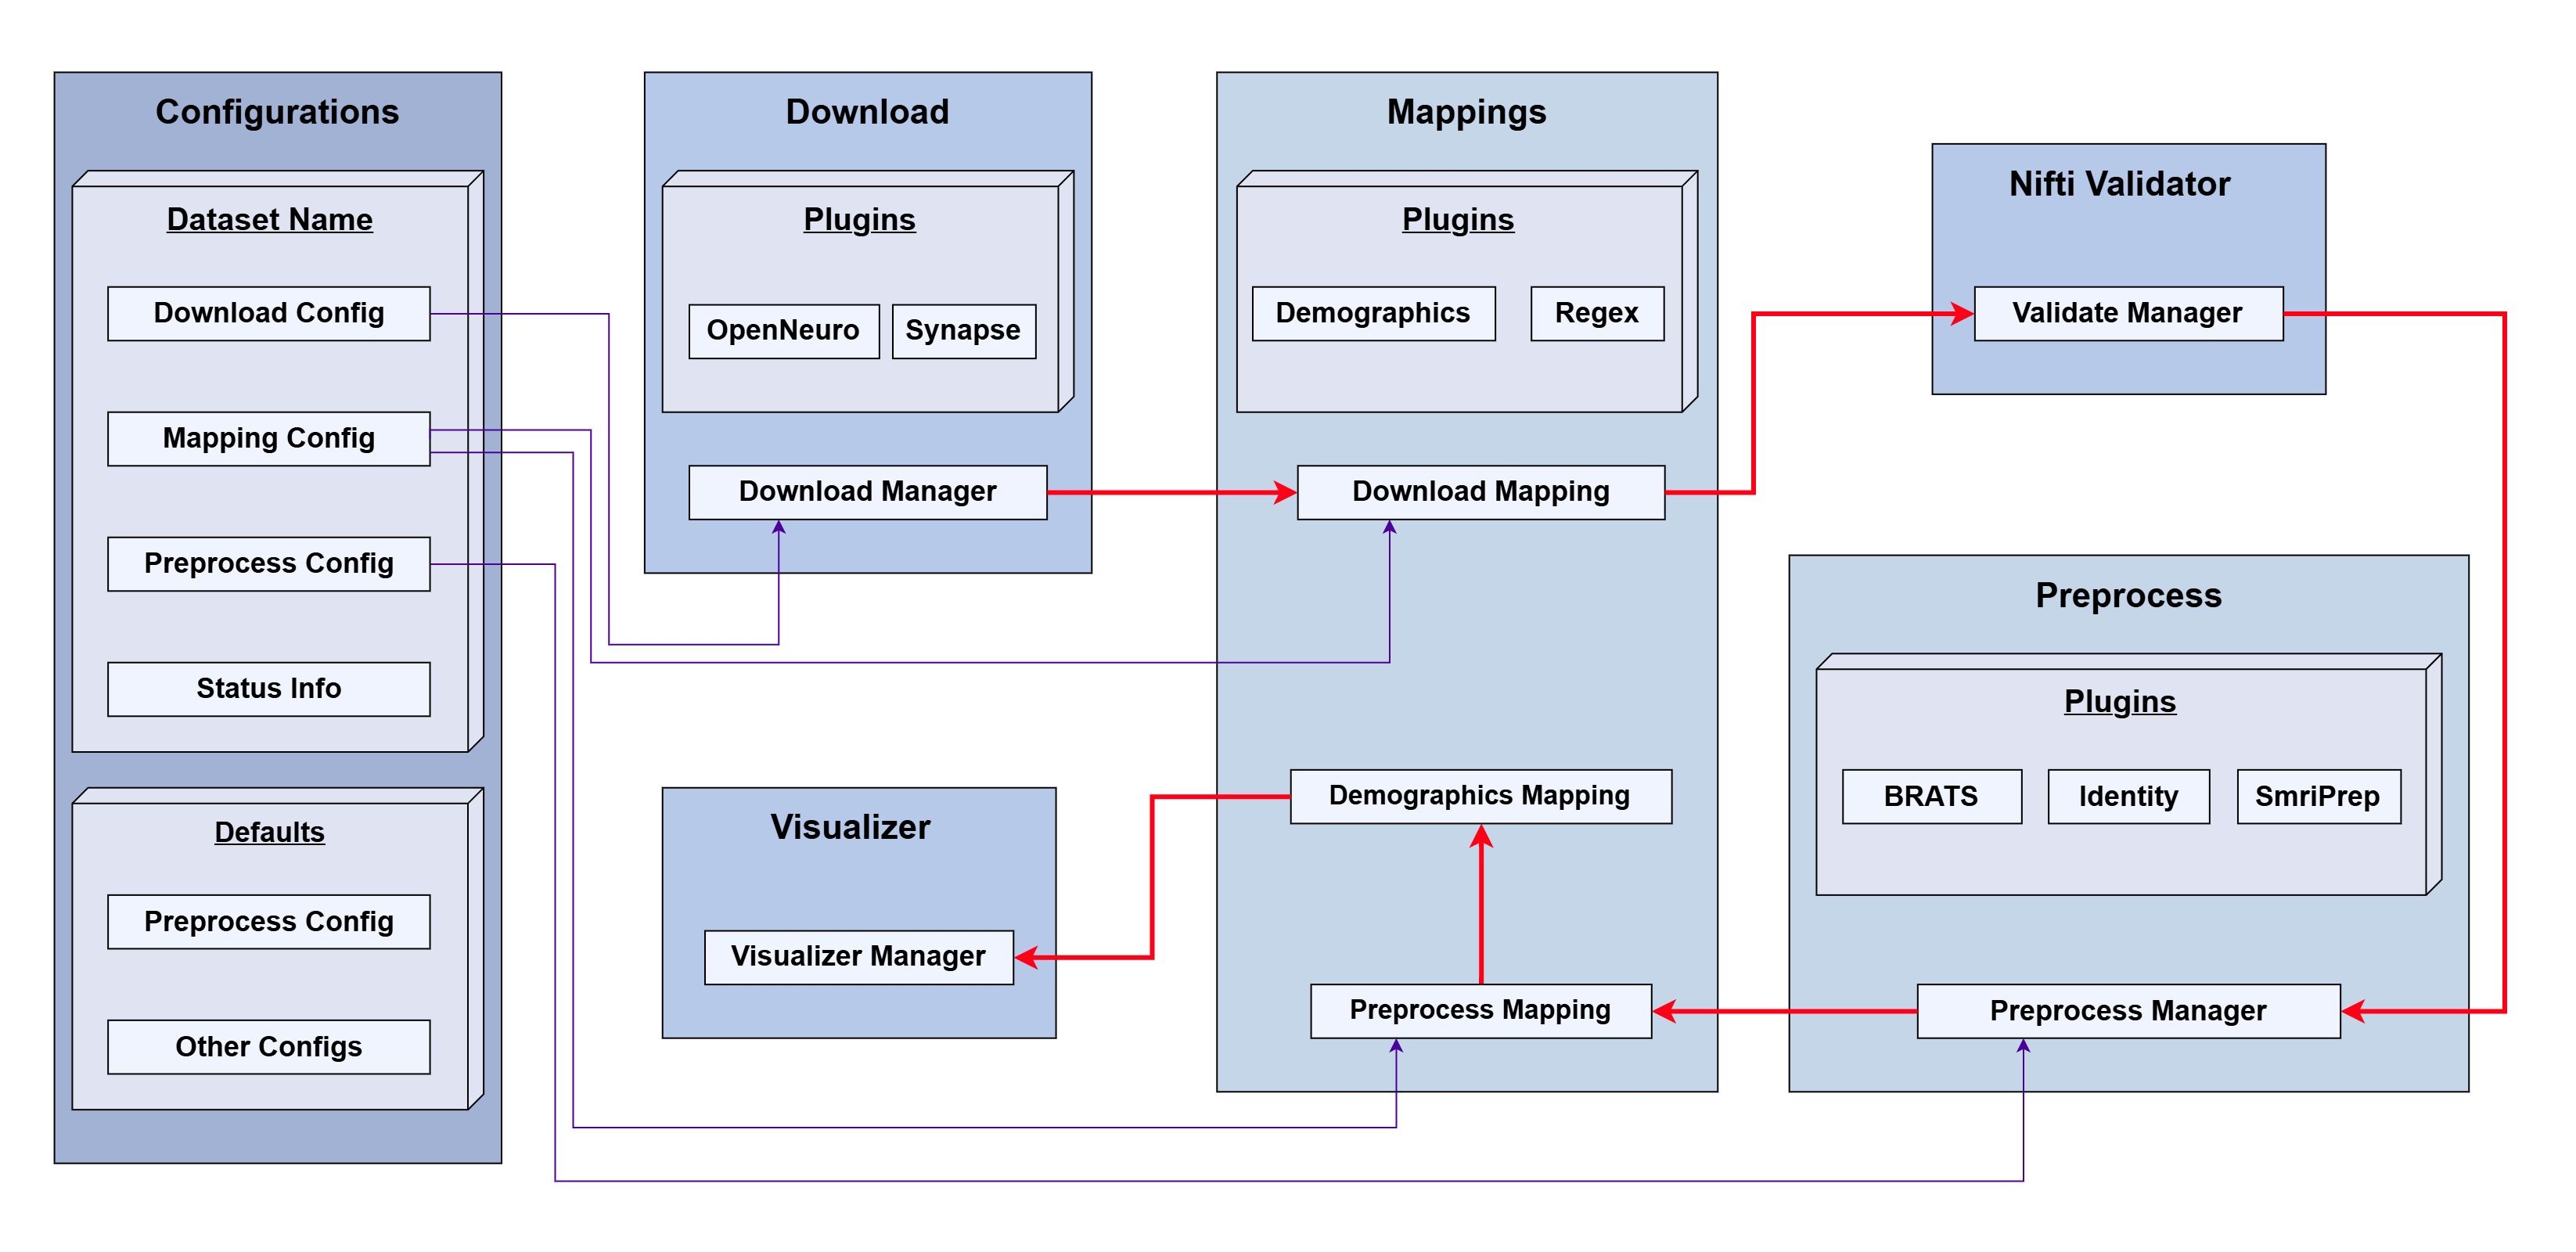
\includegraphics[width=\linewidth]{figures/architecture.png}
    \caption{
        BrainScape Framework architecture.
    }
    \label{fig:SystemArchitecture}\end{center}
\end{figure}

The pipeline workflow coordinates each module's tasks, ensuring a structured flow of data and synchronized processing. 
\textbf{Downloader Plugins}, such as the OpenNeuro downloader and Synapse downloader are used to download MRI 
data from target MRI databases and repositories.
The OpenNeuro downloader uses the \href{https://docs.aws.amazon.com/cli/latest/reference/s3/}{Amazon S3 CLI tool} to download datasets 
from OpenNeuro (\cite{markiewicz2021openneuro}) and other large-scale databases like the Human Connectome Project (HCP) (\cite{van2013wu}).
Similarly, the Synapse Downloader plugin retrieves MRI datasets from \href{https://www.synapse.org}{synapse.org}.
These plugins preserve each downloaded dataset's original folder structure, simplifying comparisons after the datasets are obtained.
\textbf{Mapper Plugins} (e.g., RegexMapper) then map the downloaded dataset files to a standardized JSON record, 
accommodating differences in dataset structure, organization, file formats, and MRI modalities based on user-defined, 
dataset-specific configuration settings.
\textbf{Validator Plugins}, such as the NIfTI Validator, check each MRI file from all of the datasets 
to detect potential errors early, thereby helping the workflow maintain high data-quality standards.

At the next stage of the pipeline, MRI preprocessing is carried out by configurable \textbf{Preprocessor Plugins}, 
each specialized for distinct imaging scenarios and requirements.
Currently, the BrainScape framework supports three primary preprocessing plugins: BraTS, sMRIPrep, and Identity. 
The BraTS preprocessor plugin implements a preprocessing pipeline closely aligned with the well-known 
Brain Tumor Segmentation challenge (BraTS) dataset preprocessing protocol (\cite{menze2014multimodal}) by 
employing the BrainLes-Preprocessing Python package (v0.4.0), publicly available at \url{https://github.com/BrainLesion/preprocessing}. 
This pipeline consists of sequential preprocessing steps, including modality co-registration 
(aligning modalities such as T2-weighted, gadolinium-enhanced T1-weighted (T1Gd), and fluid-attenuated inversion recovery (FLAIR) images to a central T1-weighted modality), 
rigid-body registration to the SRI-24 (\cite{rohlfing2010sri24}) atlas, skull stripping, and intensity normalization. 
The BrainLes-Preprocessing Python package utilizes the Advanced Normalization Tools (ANTs) 
for atlas registration and modality co-registration (\cite{tustison2021antsx}). 
Given the heterogeneous nature of datasets aggregated in BrainScape, 
we implemented a configurable priority-based selection of the central modality, 
with the default priority order set to \texttt{[T1w, T2w, T1Gd, FLAIR]}. 
For brain extraction within the BraTS pipeline, BrainLes-Preprocessing employs ``HD-BET'' (\cite{isensee2019automated}), 
an artificial neural network based tool known for robust, rapid brain extraction across diverse 
clinical MRI sequences (including T1w, T1Gd, T2w, and FLAIR modalities), pathologies, and scanner parameters. 
The HD-BET tool is utilized for brain extraction due to 
its superior accuracy and speed (typically less than 5 seconds per MRI sequence on a GPU) 
compared to widely used tools such as FSL's BET and AFNI's 3dSkullStrip (\cite{isensee2019automated, smith2000bet}).
The sMRIPrep plugin wraps the latest containerized version of the well-established sMRIPrep anatomical MRI preprocessing pipeline (\cite{esteban2021smriprep}), 
openly accessible at \url{https://www.nipreps.org/smriprep/}. 
Within sMRIPrep, anatomical images are aligned using ANTs' antsRegistration algorithm, 
enabling spatial normalization to standard templates such as MNI152 (\cite{avants2008symmetric,avants2011reproducible}).
The BrainScape sMRIPrep plugin runs the latest stable sMRIPrep Docker image (nipreps/smriprep:latest) with its default ANTs-based skull-stripping workflow, 
while disabling FreeSurfer surface reconstruction, Multimodal Surface Matching (MSM), and submillimeter reconstructions 
(\cite{esteban2021smriprep}).
Lastly, the Identity preprocessor plugin serves as a pass-through solution designed explicitly for datasets that 
have already undergone preprocessing or skull stripping. 
This approach ensures previously processed data remain unaltered, significantly simplifying the integration of diverse, 
pre-curated datasets into BrainScape.
For each dataset within the BrainScape dataset collation, 
a dataset-specific configuration file selects the appropriate preprocessing plugin. 
It also supplies all necessary parameters for that plugin, 
enabling each dataset to be preprocessed independently.

All preprocessing plugins currently available handle MRI sessions independently; 
longitudinal pipelines were deliberately omitted because our primary goal is to prepare 
individual T1w, T2w, FLAIR, and T1Gd volumes for downstream deeplearning models.
The sMRIPrep plugin was included because sMRIPrep is one of the most widely used structural MRI preprocessing pipelines, 
while the BraTS and Identity plugins align directly with our subsequent studies on AI-based brain tumour segmentation.
Nevertheless, BrainScape's modular, plugin-based architecture supports the addition of longitudinal or 
other specialized preprocessing pipelines based on the research requirements. 
To facilitate and encourage community-driven extensibility, we provide comprehensive tutorials 
on the BrainScape GitHub repository (\url{https://github.com/yasinzaii/BrainScape}), 
illustrating how researchers can develop custom plugins to meet diverse research requirements.

% \textbf{Preprocessor Plugins} (e.g., BraTS, Identity, sMRIPrep) then employ preprocessing pipelines
% that consist of specialized tasks, such as MRI registration, brain extraction, and intensity normalization. 
% For instance, the BraTS plugin uses the \href{https://github.com/BrainLesion/preprocessing}{BrainLes-Preprocessing} tool, 
% following the Brain Tumor Segmentation (BraTS) pipeline (\cite{menze2014multimodal}). 
% In the BraTS pipeline, multiple MRI modalities are co-registered to a central modality (e.g., T1w), 
% then mapped to the SR24 atlas (\cite{rohlfing2010sri24}), followed by skull stripping and image intensity normalization. 
% Datasets already preprocessed or skull-stripped can opt for simpler pipelines, 
% such as the ``Identity'' preprocessor, which applies no additional operations. 
% Other preprocessing pipelines can also be introduced as needed, maintaining the flexibility and modularity.
After preprocessing, \textbf{Mapper plugins} (e.g., RegexMapper) update the standardized JSON record 
with the preprocessed MRI files. The \textbf{Demographics Mapper} plugin then appends relevant demographic 
and clinical fields (e.g., age, sex, diagnosis) to each subject record, thereby producing a unified 
resource that integrates both anatomical and demographic information.

BrainScape framework's modular, plugin-based architecture supports plugin swaps via configuration files, 
eliminating the need to alter the codebase. As a result, researchers can 
readily include additional plugins supporting specialized pipelines for their unique study requirements. 
BrainScape's pipeline workflow and configurable plugins provide a robust, adaptable system for MRI data management.


\subsection{Experimental Setup and Performance Measurement}

We conducted experiments on a local workstation equipped with a 13th Generation Intel Core i9-13900K CPU 
and an NVIDIA GeForce RTX 4070 Ti GPU (12GB VRAM). 
The CPU has 24 physical cores running at a speed of up to 5.8\,GHz. 
The pipeline was tested using Python 3.11 on Ubuntu 22.04.
To evaluate the BrainScape framework pipeline, 
we selected the publicly available \href{https://openneuro.org/datasets/ds003717}{VASP dataset} (\cite{peelle2022increased}) from OpenNeuro, 
which includes T1w and T2w MRI scans for 60 subjects (120 MRI scans in total). 

We utilized several Python packages to capture performance metrics: 
``time'' for measuring wall-clock time, 
\href{https://docs.python.org/3/library/resource.html}{resource} for computing CPU time,
\href{https://pypi.org/project/psutil/}{psutil} to calculate average CPU utilization, 
\href{https://pypi.org/project/pynvml/}{pynvml} for GPU usage and memory consumption, and 
\href{https://pypi.org/project/codecarbon/}{CodeCarbon} to estimate electricity consumption (kWh) and CO$_2$-equivalents (CO$_2$eq) emissions, 
using the carbon intensity data from New Zealand's local electricity grid.

Currently, the pipeline is designed to process datasets sequentially. 
Nevertheless, its modular design and configurable workflow support running multiple datasets in parallel 
which will be effective in reducing the overall wall-clock time.


\subsection{Hardware and Software Requirements}

BrainScape framework is designed to run on standard 64-bit Linux distributions and has been tested on Ubuntu 22.04. 
Additionally, it supports Windows 10 and 11 through the \href{https://learn.microsoft.com/en-gb/windows/wsl}{Windows Subsystem for Linux 2 (WSL2)}.
Essential software prerequisites include \href{https://www.anaconda.com/docs/getting-started/miniconda/main}{Miniconda} for managing 
a dedicated Python (version 3.11) environment  
and \href{https://docs.aws.amazon.com/cli/latest/userguide/getting-started-install.html}{AWS CLI v2} for accessing and 
downloading MRI data from Amazon S3-hosted repositories, such as \href{https://openneuro.org/}{OpenNeuro}. 
A GPU is recommended to accelerate the computationally intensive preprocessing task of skull stripping 
performed by the HD-BET brain-extraction tool (\cite{isensee2019automated}) in the BraTS plugin. 
However, a GPU is not mandatory; CPU-only systems can still run the pipeline, though they will take longer to preprocess.
Furthermore, BrainScape has been successfully deployed and tested on the 
\href{https://www.nesi.org.nz/}{New Zealand eScience Infrastructure (NeSI)} 
high-performance computing (HPC) platform, demonstrating its scalability and compatibility with cluster computing environments. 
NeSI compute nodes run Rocky Linux, a widely used Red Hat-compatible operating system standard across large-scale HPC facilities. 
Detailed installation instructions, configuration guidelines, and execution documentation are available on
the \href{https://github.com/yasinzaii/BrainScape}{BrainScape GitHub} repository.



\FloatBarrier
\section{Results}
\subsection{Overall Dataset Composition}

The BrainScape dataset includes four anatomical MRI contrasts, i.e., T1-weighted (T1w), T2-weighted (T2w), 
gadolinium-enhanced T1-weighted (T1Gd), and fluid-attenuated inversion recovery (FLAIR).
Furthermore, it integrates \NumDatasets\ datasets from diverse open-source repositories and individual research studies. 
After quality control and visual inspection (e.g., excluding MRIs with artifacts, corrupted and poor-quality scans), 
\TotalNumSubjects\ unique subjects remain in the database, yielding \TotalNumMRIs\ MRI scans overall. 

Among these, \TotalTOneMRIs\ are T1w, \TotalTTwoMRIs\ are T2w, \TotalTOneGdMRIs\ are T1Gd, and \TotalFlairMRIs\ are FLAIR. 
As summarized in Table~\ref{TableMriModDistribution}, the distribution of modalities is uneven, 
with T1w scans representing a larger share of the total MRIs. 
Yet, the inclusion of T2w and FLAIR scans extends the framework's utility to 
applications where multi-contrast data are essential (e.g., lesion analysis, tissue segmentation).

\begin{table}
    \centering
    \begin{threeparttable}
        \caption{MRI Modality Distribution.}
        \label{TableMriModDistribution}
        \begin{tabular}{lcc}
            \toprule
            \textbf{Modality} & \textbf{Count} & \textbf{(\% of Total)} \\
            \midrule
            T1w    & \TotalTOneMRIs\    & \TOnePercent \\
            T2w    & \TotalTTwoMRIs\    & \TTwoPercent \\
            T1Gd    & \TotalTOneGdMRIs\    & \TOneGdPercent \\
            FLAIR  & \TotalFlairMRIs\   & \FlairPercent \\
            \bottomrule
        \end{tabular}
    \end{threeparttable}   
\end{table}
    
As shown in Table~\ref{TableMriModDistribution}, T1w scans are substantially more common than T2w, T1Gd and FLAIR scans.
Among the \NumDatasets\ datasets included in BrainScape, only one dataset (BRATS) provides T1Gd MRI scans. 
T2w MRI scans are available in \NumDatasetsWithTTwoScans\ datasets, 
FLAIR scans in \NumDatasetsWithTFlairScans\ datasets, 
and T1w scans in \NumDatasetsWithTToneScans\ datasets.
On the other hand, the number of sessions per subject also varies, 
ranging from a single scan per subject to multiple scans per subject. The BrainScape dataset 
retains session information and the original dataset structures, ensuring flexibility 
for downstream analyses. For complete details of each individual dataset and the available
MRI modalities, refer to the Supplementary Material (Table 1).

Since T1w scans are more common than other modalities, 
analyses relying primarily on T2w, T1Gd, or FLAIR scans may include fewer subjects. 
However, the availability of multimodal MRI scans remains valuable for specialized clinical studies or advanced modeling tasks such as lesion segmentation. 
Researchers can leverage BrainScape's flexibility to utilize the entire dataset or a subset of the dataset, depending on the specific requirements of the study.

\begin{figure}[ht]
    \centering
    \includegraphics[width=\linewidth]{figures/example_multimodal_mri.png} 
    \caption{
        Multimodal MRIs of three subjects from different datasets with each subject having T1w, T2w, and FLAIR modalities. 
        The vertical axis (Y-axis) lists each subject by its source dataset identifiers (detailed in the Supplementary Material), 
        while the horizontal axis shows axial, coronal, and sagittal slices for each modality. 
        Here, the subject from the ``QTAB'' dataset is a 10-year-old female, 
        the subject from ``MPLMBB'' is a male aged between 65-70, 
        and the subject from ``ARCD'' is a 40-year-old male with a stroke. 
    }
    \label{fig:ExampleMultimodal}
\end{figure}

The MRI scans aggregated in the BrainScape dataset originate from scanners with diverse hardware, manufacturers, and magnetic field strengths.
Among the \TotalNumMRIs\ MRIs included, MRI scanner metadata was available for 24508 scans (52.61\%), 
while scanner information for the remaining 22075 scans (47.39\%) was missing (see Supplementary Table 2). 
Furthermore, among the 24508 MRIs with scanner information, 22089 MRIs had magnetic field strength information available.
MRI data originated primarily from three major manufacturers (Siemens, Philips, and GE), 
with Siemens scanners being the most prevalent across all modalities. 
The dataset predominantly includes 3.0 Tesla (T) MRI scanners (18147 scans), followed by 1.5T (2584 scans), 
4.0T (1301 scans), and a small subset from 7.0T scanners (57 scans). 
The BrainScape dataset contains scans from various manufacturers, models, and field strengths, 
mirroring the variability seen in clinical and research imaging. 
This diversity makes the BrainScape dataset an excellent resource for training AI models that are both robust and generalizable.
Scanner metadata, including the manufacturer name, model details, and field strength information, is stored in the BrainScape JSON record.

Figure~\ref{fig:ExampleMultimodal} illustrates how BrainScape integrates multimodal MRI data 
from diverse heterogeneous datasets, with varying participant demographics and clinical profiles. 
Our framework effectively combines these heterogeneous datasets and enables researchers 
to examine both healthy individuals and those with specific conditions (such as stroke). 
Moreover, BrainScape preserves the demographic and clinical metadata, allowing researchers 
to readily filter or subgroup images by attributes like age, sex, or clinical diagnosis. 
This flexibility supports a wide range of analyses, from large-scale population studies 
to more focused clinical investigations.


\subsubsection{Demographics Information}

A total of \TotalSubjectsIncludedAfterInspectionCount\ subjects were included after inspection 
from a total of \NumDatasets\ datasets. Of these, \TotalSubjectsWithDemographicsInfoCount\ subjects 
have demographic information, while \TotalSubjectsWithoutDemographicsInfoCount\ 
subjects lack any recorded demographic details. The demographic data include age, sex, race, handedness, education level, 
socio-economic status, body mass index, and brain disorders. Table~\ref{DemographicsOverviewTable} provides a comprehensive 
overview of the availability of each demographic field across all of the datasets.

\begin{table}[h!]
    \centering
    \begin{threeparttable}
        \caption{Count of Subjects with Each Demographic Field}
        \label{DemographicsOverviewTable}
        \setlength{\tabcolsep}{45pt}%
        
        \begin{tabular}{@{}ll}
            \toprule
            \textbf{Demographic Field} & \textbf{Number of Subjects} \\
            \midrule
            Specific Age & \TotalSubjectsWithAgeCount\ \\
            Age Range & \TotalSubjectsWithAgeGroupCount\ \\
            Sex & \TotalSubjectsWithSexCount\ \\
            Handedness & \TotalSubjectsWithHandednessCount\ \\
            Race & \TotalSubjectsWithRaceCount\ \\
            Education & \TotalSubjectsWithEducationCount\ \\
            Socio-Economic Status & \TotalSubjectsWithSocioEconomicCount\ \\
            Body Mass Index & \TotalSubjectsWithBodyMassIndexCount\ \\
            Brain Disorders & \TotalSubjectsWithDisordersCount\ \\
            No Demographics & \TotalSubjectsWithoutDemographicsInfoCount\ \\
            \bottomrule
        \end{tabular}
        
        %\begin{tablenotes}[flushleft]\footnotesize
        %    \item[${a}$] Basic counts of demographic coverage across the dataset.
        %\end{tablenotes}
    \end{threeparttable}
\end{table}

It is evident that age (or age range) and sex are among the most crucial and commonly analyzed demographics. 
According to Table~\ref{DemographicsOverviewTable}, \TotalSubjectsWithAgeCount\ subjects have an explicit age value, 
\TotalSubjectsWithAgeGroupCount\ subjects include a recorded age range label, and \TotalSubjectsWithSexCount\ subjects have sex information. 
Of these, \TotalSubjectsWithAgeAgeGroupSexCount\ subjects possess both age (or age range) and sex information.

\begin{figure}[ht]
    \centering
    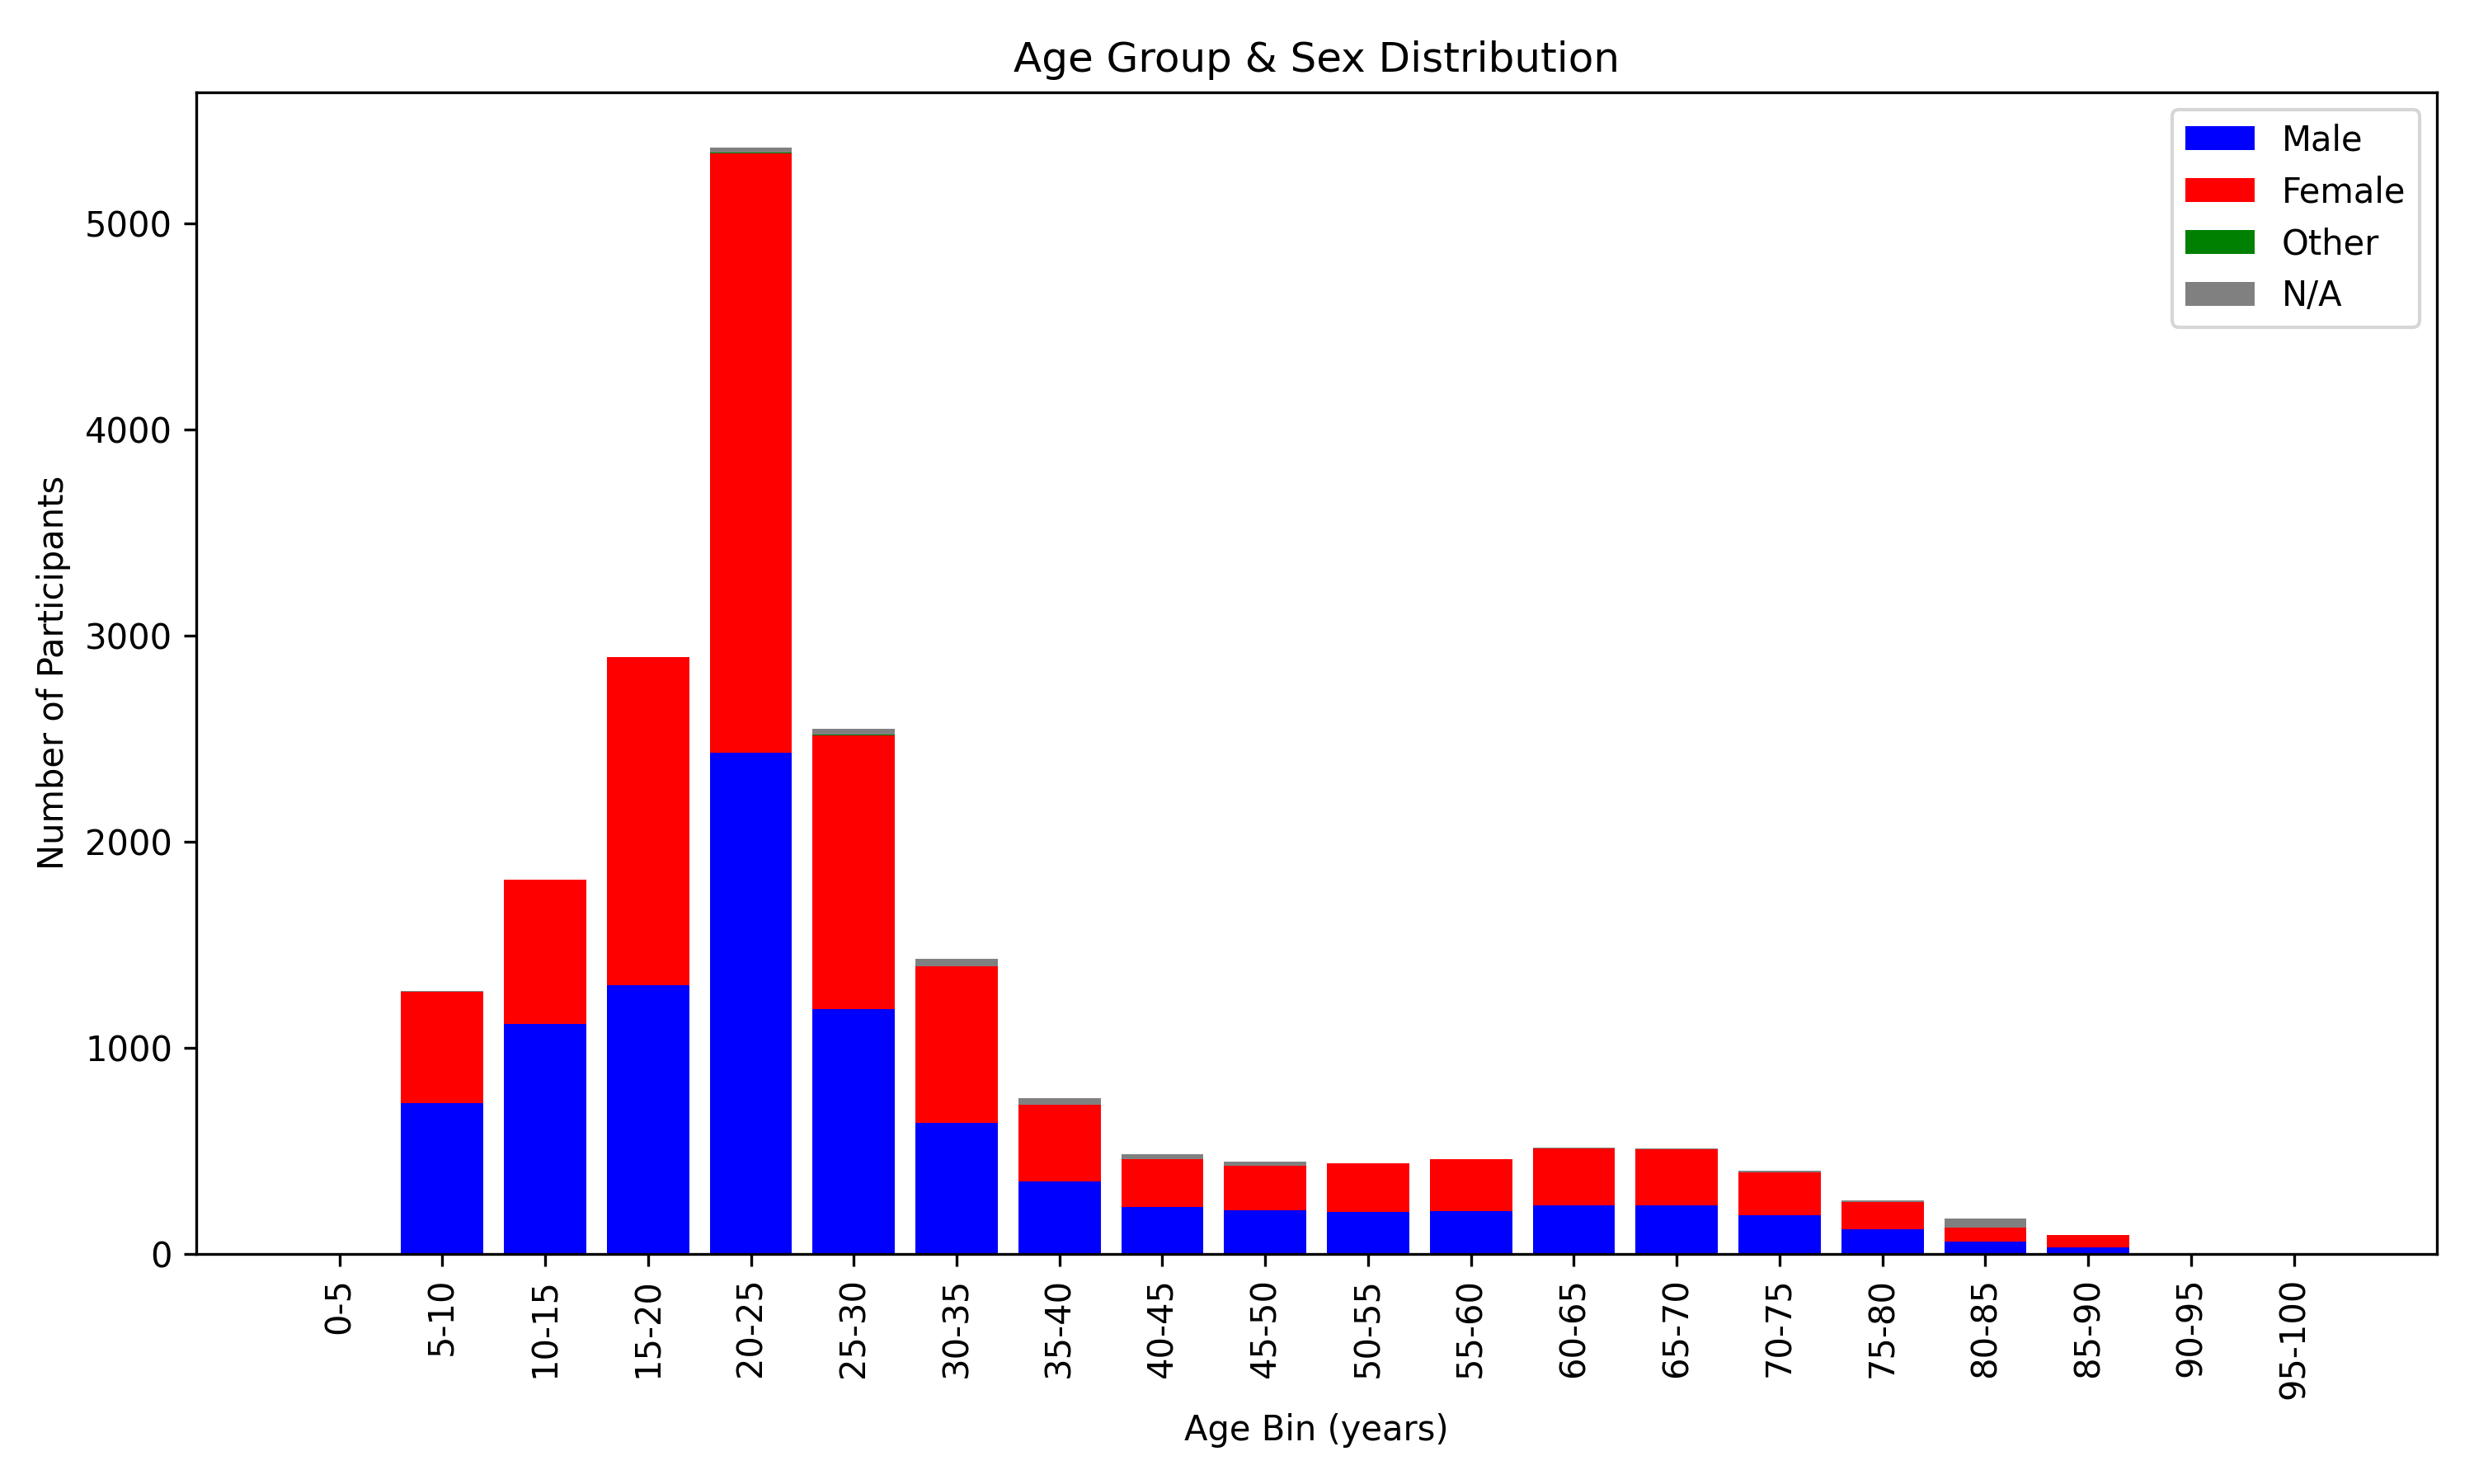
\includegraphics[width=\linewidth]{figures/age_group_sex_histogram} 
    \caption{Histogram of Age (or Age Ranges) by Sex. Each bar represents a bin of age or an age range, subdivided by sex categories (male, female, n/a).}
    \label{HistogramAgeSexFigure}
\end{figure}

\noindent
Figure~\ref{HistogramAgeSexFigure} presents a histogram illustrating how the dataset's age distribution is subdivided by sex categories. 
Specifically, the histogram organizes age (or age range) into bins along the horizontal axis, whereas the vertical bars 
representing the participants count, color-coded to indicate the sex categories: ``male'', ``female'', and ``n/a''. Note: \TotalSubjectsWithSexCountWithoutAgeInfo\ 
subjects who have only sex information and lack age or age range information are omitted from the histogram.

Overall, the mean age (excluding entries with only age range data) is \TotalSubjectsMeanAgeValue\ (SD = \TotalSubjectsStandardDevAgeValue{}). 
By categorizing individual ages into bins, as illustrated in Figure~\ref{HistogramAgeSexFigure}, the median age range is determined to be \TotalSubjectsMedianAgeGroupValue\ years.
The sex distribution among subjects with available sex information, 
regardless of age data, includes \TotalSubjectsWithMaleSexCount\ males 
and \TotalSubjectsWithFemaleCount\ females, 
totaling \TotalSubjectsWithMalePlusFemaleCount\ subjects. 

\begin{table}[ht]
    \centering
    \begin{threeparttable}
        \caption{Distribution of Demographic Variables}
        \label{additional_demographics}
        \begin{tabular}{@{}lcccc@{}}
            \toprule
            \textbf{Variable} & \textbf{Category/Level} & \textbf{Count (n)} & \textbf{Percentage (\%)} & \textbf{Total (n)} \\
            \midrule
            \textbf{Race}   & White & \TotalSubjectsWithWhiteRaceCount & \TotalSubjectsWithWhiteRacePercentage & \TotalSubjectsWithRaceCount \\
                            & Black & \TotalSubjectsWithBlackRaceCount & \TotalSubjectsWithBlackRacePercentage & \\
                            & Asian & \TotalSubjectsWithAsianRaceCount & \TotalSubjectsWithAsianRacePercentage & \\
                            & American Indian/Alaska Native & \TotalSubjectsWithAmericanIndianAlaskanRaceCount & \TotalSubjectsWithAmericanIndianAlaskanRacePercentage & \\
                            & Hawaiian/Pacific Islander & \TotalSubjectsWithHawaiianPacificIslanderRaceCount & \TotalSubjectsWithHawaiianPacificIslanderRacePercentage & \\
                            & Two or More Races & \TotalSubjectsWithTwoOrMoreRaceCount & \TotalSubjectsWithTwoOrMoreRacePercentage & \\
                            & Other & \TotalSubjectsWithOtherRaceCount & \TotalSubjectsWithOtherRacePercentage & \\
            \textbf{Handedness} & Right (R) & \TotalSubjectsWithRightHandednessCount & \TotalSubjectsWithRightHandednessPercentage & \TotalSubjectsWithHandednessCount \\
                                & Left (L) & \TotalSubjectsWithLeftHandednessCount & \TotalSubjectsWithLeftHandednessPercentage & \\
                                & Ambidextrous (A) & \TotalSubjectsWithAmbidextrousHandednessCount & \TotalSubjectsWithAmbidextrousHandednessPercentage &  \\
            \textbf{Education} & Low (Primary/HS) & \TotalSubjectsWithLowEducationCount & \TotalSubjectsWithLowEducationPercentage & \TotalSubjectsWithEducationCount\\ 
                               & Medium (College) & \TotalSubjectsWithMediumEducationCount & \TotalSubjectsWithMediumEducationPercentage & \\
                               & High ($\geq$ Bachelors) & \TotalSubjectsWithHighEducationCount & \TotalSubjectsWithHighEducationPercentage & \\
            \textbf{Socio-Economic Status}  & Low & \TotalSubjectsWithLowEconomicCount & \TotalSubjectsWithLowEconomicPercentage & \TotalSubjectsWithSocioEconomicCount\\
                                            & Medium & \TotalSubjectsWithMediumEconomicCount & \TotalSubjectsWithMediumEconomicPercentage & \\
                                            & High & \TotalSubjectsWithHighEconomicCount & \TotalSubjectsWithHighEconomicPercentage & \\
            \bottomrule
        \end{tabular}
        \begin{tablenotes}[flushleft]\footnotesize
            \item[${a}$] Frequencies and percentages of race, handedness, education, and socio-economic status.
        \end{tablenotes}
    \end{threeparttable}
\end{table}

Beyond age and sex, additional demographic information such as race, handedness, education level, 
and socio-economic status was available only for subsets of participants, 
with notable variability across datasets (see Table~\ref{additional_demographics}). 
Out of \TotalSubjectsWithRaceCount\ subjects with available race information, 
the majority identified as White (\TotalSubjectsWithWhiteRaceCount; \TotalSubjectsWithWhiteRacePercentage\%), 
followed by Black or African American (\TotalSubjectsWithBlackRaceCount; \TotalSubjectsWithBlackRacePercentage\%) 
and Asian (\TotalSubjectsWithAsianRaceCount; \TotalSubjectsWithAsianRacePercentage\%). 
Handedness information, available for \TotalSubjectsWithHandednessCount\ subjects, 
indicated a majority were right-handed (\TotalSubjectsWithRightHandednessCount; \TotalSubjectsWithRightHandednessPercentage\%), 
while left-handed (\TotalSubjectsWithLeftHandednessCount; \TotalSubjectsWithLeftHandednessPercentage\%) 
and ambidextrous (\TotalSubjectsWithAmbidextrousHandednessCount; \TotalSubjectsWithAmbidextrousHandednessPercentage\%) participants were less common.

Educational information for \TotalSubjectsWithEducationCount\ subjects were categorized into three distinct groups: low, medium, and high. 
The low education group (\TotalSubjectsWithLowEducationCount\ subjects, \TotalSubjectsWithLowEducationPercentage\%) includes participants 
who completed primary education or obtained a high school diploma as their highest education level. 
The medium education group (\TotalSubjectsWithMediumEducationCount\ subjects, \TotalSubjectsWithMediumEducationPercentage\%) consists 
of participants who completed some form of post-secondary education below a four-year degree, such as college, a diploma, or an Associate's Degree. 
The higher education category (\TotalSubjectsWithHighEducationCount\ subjects, \TotalSubjectsWithHighEducationPercentage\%) comprises individuals 
who have completed at least a Bachelor's degree, including Master's or doctoral degrees (PhD). 
Similarly, socioeconomic status, available for \TotalSubjectsWithSocioEconomicCount\ subjects, is categorized into 
low (\TotalSubjectsWithLowEconomicCount\ subjects, \TotalSubjectsWithLowEconomicPercentage\%), 
medium (\TotalSubjectsWithMediumEconomicCount\ subjects, \TotalSubjectsWithMediumEconomicPercentage\%), and high (\TotalSubjectsWithHighEconomicCount\ subjects, 
\TotalSubjectsWithHighEconomicPercentage\%) groups.


\subsubsection{Participants from clinical cohorts}

A total of \TotalSubjectsWithDisordersCount\ participants that are part of the BrainScape dataset have been diagnosed with disorders.
These disorders include Neurological disorders (Stroke, Prosopagnosia, Dysembryoplastic Neuroepithelial Tumor (DNT), Gliosis, and Epilepsy), Psychiatric disorders (Depression and Schizophrenia)
and Developmental disorders (Attention-Deficit/Hyperactivity Disorder (ADHD) and Autism Spectrum Disorder (ASD)). 
Table~\ref{brain_disorders} lists the number of subjects diagnosed with each disorder among 
the overall \TotalSubjectsIncludedAfterInspectionCount\ individuals. 

\begin{table}[ht]
    \centering
    \begin{threeparttable}
        \caption{Number of Subjects with specific Disorders}
        \label{brain_disorders}
        \begin{tabular}{@{}lc@{}}
            \toprule
            \textbf{Disorder} & \textbf{Number of Subjects} \\
            \midrule
            Stroke & \SubjectsWithStrokeCount\ \\
            Acute Ischemic Stroke & \SubjectsWithAcuteIschemicStrokeCount\ \\
            Schizophrenia & \SubjectsWithSchizophreniaCount\ \\
            Depression & \SubjectsWithDepressionCount\ \\
            ADHD & \SubjectsWithADHDCount\ \\
            ASD & \SubjectsWithASDCount\ \\
            Bipolar Disorder & \SubjectsWithBIPOLARCount\ \\
            Prosopagnosia & \SubjectsWithProsopagnosiaCount\ \\
            Epilepsy & \SubjectsWithEpilepsyCount\ \\
            Focal Epilepsy & \SubjectsWithFocalEpilepsyCount\ \\
            Tumor & \SubjectsWithTumorCount\ \\
            Gliosis & \SubjectsWithGLCount\ \\           
            DNT & \SubjectsWithDNTCount\ \\
            Aneurysm & \SubjectsWithAneurysmCount\ \\
            \bottomrule
        \end{tabular}
        \begin{tablenotes}[flushleft]\footnotesize
            \item[${a}$] Only participants who tested \texttt{Y} (Yes) for each disorder are counted here.
        \end{tablenotes}
    \end{threeparttable}
\end{table}

\noindent
Table~\ref{brain_disorders} highlights that \SubjectsWithStrokeCount\ participants have been 
diagnosed with stroke, \SubjectsWithEpilepsyCount\ with epilepsy, and so on. 
The \SubjectsWithFocalEpilepsyCount\ subjects with focal epilepsy consist of \SubjectsWithFCDCount\ subjects 
with focal cortical dysplasia and \SubjectsWithHSCount\ subjects with hippocampal sclerosis.
In total, \TotalSubjectsWithDisordersCount\ participants have at least one neurological, psychiatric, or developmental disorder.


\subsubsection{Quality Control and Visual Inspection}

All MRI datasets included in this study underwent visual inspection to identify and exclude scans presenting various artifacts, 
including motion artifacts, susceptibility distortions, aliasing (wrap-around) artifacts, and Gibbs ringing artifacts. 
Similarly, subjects with poorly defaced MRIs, where portions of the brain were inadvertently removed, were excluded. For transparency and 
traceability, any scan failing visual quality checks is listed in the corresponding dataset's metadata, enabling researchers to audit, 
revisit, or reverse these exclusions if required.

This process has thus far resulted in the removal of \TotalNumSubjectsRemoved\ subjects across \TotalNumDatasetsWithSubjectsRemoved\ datasets 
from the total of \NumDatasets\ included in the repository. 
Additionally, \NumDatasetsAlreadySkullStripped\ datasets out of the total \NumDatasets\ have brain MRIs that were already skull-stripped. 
However, we opted to exclude scans with incomplete skull stripping, such as those illustrated in Figure \ref{dropped_subject}. 
Reprocessing datasets that contain both fully and partially skull-stripped MRIs with the default BraTS preprocessing plugin, 
which uses HD-BET brain-extraction tool (\cite{isensee2019automated}), results in over-erosion of brain tissue during brain extraction.
We decided to drop incomplete skull-stripped scans from such datasets to keep a single default BraTS preprocessing pipeline for the BrainScape dataset release, 
and because this issue affected only a small subset of subjects (approximately 130 subjects).
Figure~\ref{dropped_subject} illustrates examples of the excluded MRI scans, highlighting the types of artifacts and issues that led to their removal. By making the exclusion 
criteria explicit and open to re-evaluation by the neuroscience community, we reduce the risk of perpetuating errors and encourage collaborative quality assurance, 
ultimately enhancing the overall integrity and reproducibility of the dataset.


\begin{figure}[htbp]\begin{center}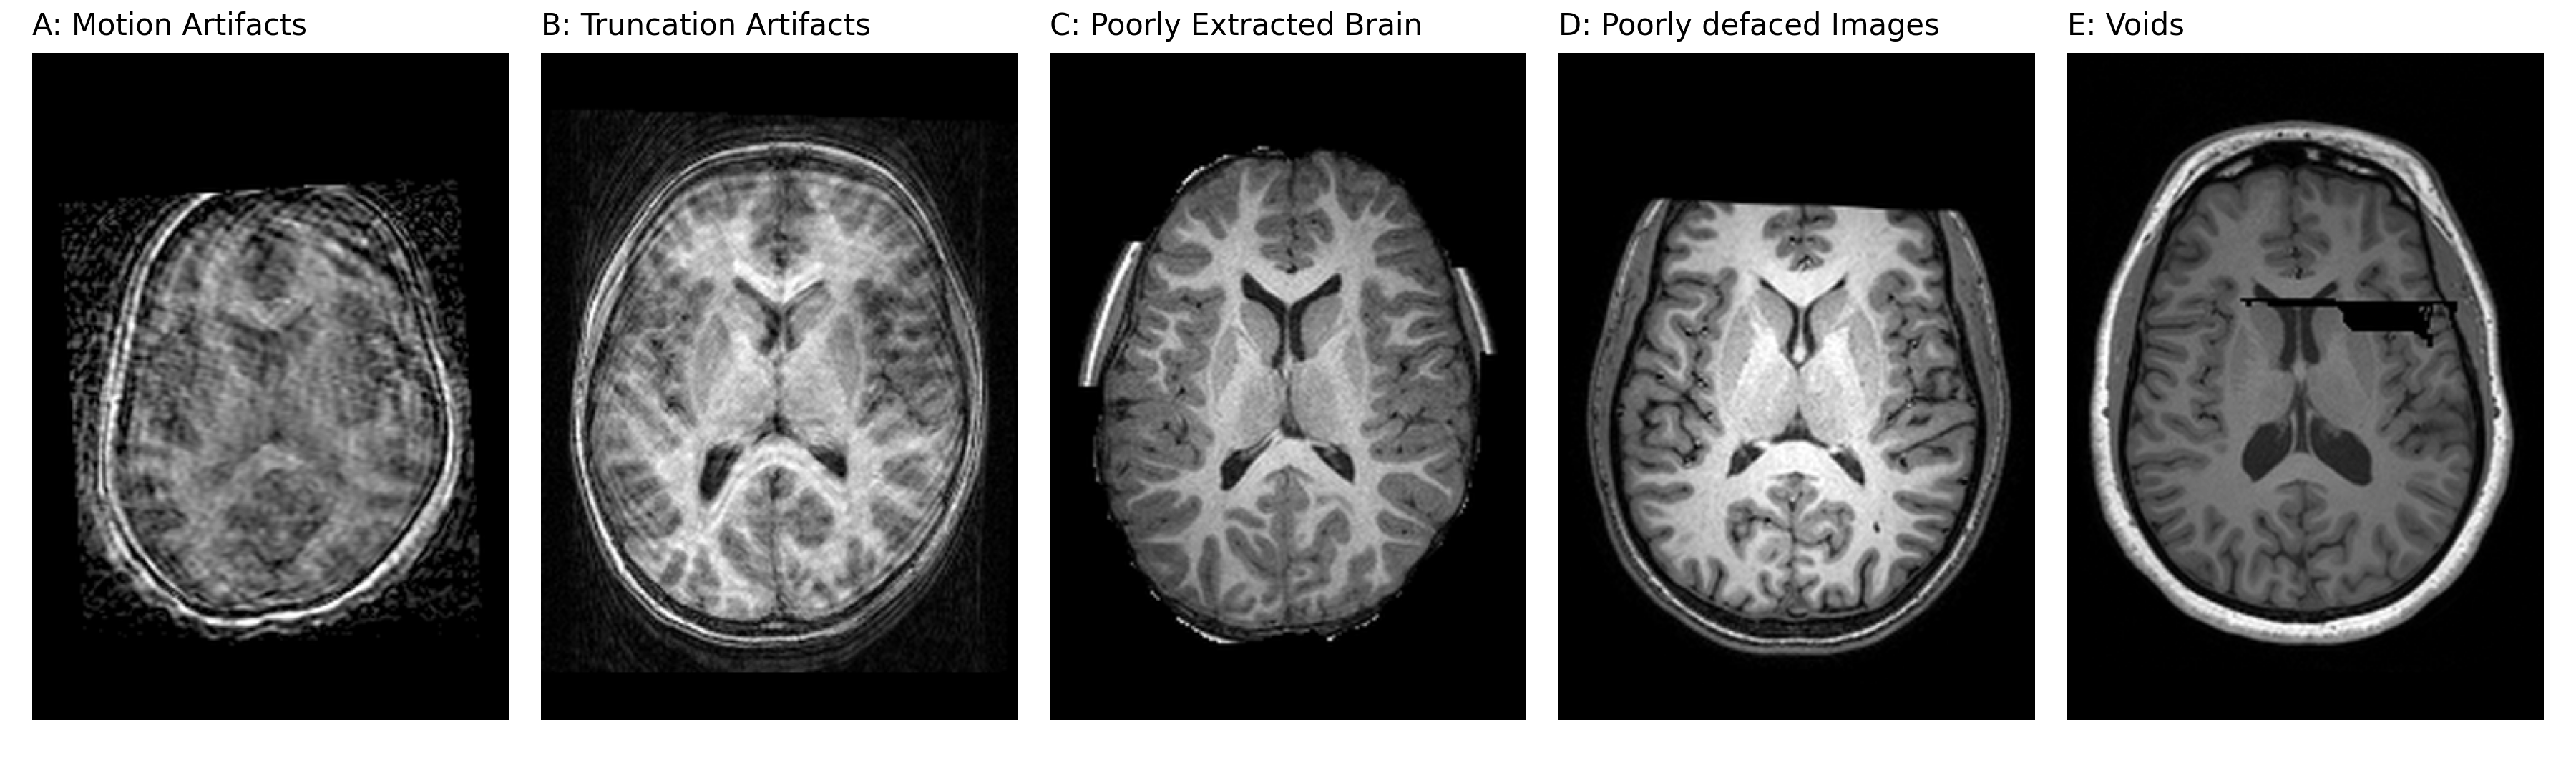
\includegraphics[width=\linewidth]{figures/dropped_subjects.png}
    \caption{
        Examples of MRI scans excluded during visual quality inspection:
        (A) Motion artifacts, 
        (B) Gibbs ringing artifact (truncation artifact), 
        (C) Poorly extracted brain regions, 
        (D) Inadequate defacing with cropped brain regions, 
        and (E) Missing or void pixels.
    }
    \label{dropped_subject}\end{center}
\end{figure}


\subsection{Computational Performance and Carbon Footprint}

The BrainScape framework completed the full workflow for the VASP dataset (120 MRI scans) in approximately 33.3\,minutes of wall-clock time. 
The recorded CPU utilization was only 21.85\%, reflecting the predominantly sequential structure of our current implementation. 
In total, the pipeline took 228\,minutes of CPU time across the 24 CPU cores, indicating further room for parallelization. 
Future updates to BrainScape are expected to enable running multiple datasets concurrently, 
which can significantly shorten wall-clock time and increase overall efficiency.
Real-time monitoring of GPU resources revealed that usage peaked during skull stripping (during preprocessing), 
with memory consumption reaching about 5406\,MB (44\% of the available 12\,GB). 
Outside of these intensive operations, the GPU remained largely idle, resulting in an average utilization 
of 24.78\% throughout the entire workflow. 
Incorporating additional datasets is expected to proportionally increase wall-clock time and CPU time.

We also evaluated the pipeline's environmental impact by considering local grid emission factors in New Zealand. 
Over the entire run on the VASP dataset, the pipeline consumed an estimated 0.07065 kilowatt-hours (kWh) of electricity, corresponding to 
0.00796\,kg of CO\textsubscript{2}eq emissions. 
0.07065 kWh is roughly the energy needed to keep a 10 W LED lamp on for seven hours, 
or to run a typical 1.5 kW space heater for a little under three minutes.
As more datasets are included, the energy consumption and 
carbon footprint may rise proportionally; however, workflow parallelization can help maintain 
reasonable total run times and minimize ecological impact. By documenting these performance metrics, we highlight 
the computational overhead and the opportunity to reduce processing times and emissions through concurrent dataset handling. 
We anticipate that implementing parallel dataset processing pipelines will improve BrainScape's computational performance and carbon footprint.


\FloatBarrier
\section{Discussion}
In this paper, we introduce BrainScape, an easy-to-use resource that combines an open-source, 
plugin-based software framework with a collated dataset distributed as a curated set of 
dataset-specific configuration files.
BrainScape simplifies the downloading, management, aggregation, and preprocessing of publicly available anatomical MRI data, 
making it straightforward for researchers to regenerate standardized, analysis-ready datasets.
BrainScape addresses known challenges associated with aggregating multimodal MRI datasets, 
including the fragmentation of specialized clinical data, incompatible dataset formats and organization, 
lack of automated data-handling workflows, and inconsistencies in demographic and clinical metadata.
BrainScape integrates heterogeneous MRI datasets while preserving each dataset's original structure, 
subject organization, and licensing details.
This design choice minimizes the risks of data duplication, data loss, and inadvertent bias, 
enabling researchers to easily and reliably merge data from multiple sources 
for more comprehensive analyses.

One of the strengths of BrainScape is its flexibility and scalability. 
The configurable and modular plugin-based architecture of the BrainScape framework enables 
seamless integration of new data sources, imaging modalities, and preprocessing pipelines without requiring any modifications to the core codebase.
Researchers can add new multimodal MRI datasets by including new configuration files. 
Additionally, the BrainScape framework provides the flexibility to include plugins for downloading data from other open source MRI databases and  
specialized preprocessing plugins for specific studies that may consist of custom preprocessing pipelines.
This design facilitates an environment of continuous improvement and customization.
We integrate \NumDatasets\ diverse datasets, demonstrating the framework's scalability 
and capability to handle large-scale data aggregation.
Furthermore, BrainScape's ability to trace each file back to its source and maintain 
dataset-specific configurations demonstrates reproducibility by ensuring that the inclusion criteria, 
quality-control outcomes, and plugin parameters are recorded in a transparent and standardized manner.

By automating data downloading, mapping, validation, and preprocessing, BrainScape framework reduces the 
manual labor required for large-scale, multi-site data pooling. Researchers can therefore shift 
their focus away from tedious preparation tasks and concentrate on analysis, interpretation, and theory development. 
This is particularly helpful for deep learning and machine learning applications, where model 
performance benefits from the diversity and volume of training data (\cite{dishner2024survey}). Beyond aggregating diverse MRI scans, 
BrainScape also supports attaching demographic fields (such as age, sex, handedness, and clinical status), enabling 
researchers to build inclusive datasets that capture control and patient cohorts. 
This diversity is particularly crucial for rare phenotypes and targeted clinical cohorts, 
which may be overlooked in large-scale aggregated datasets yet offer critical insights into neurological function and pathology (\cite{thompson2014enigma}).

The BrainScape framework is designed to interoperate seamlessly with the broader neuroinformatics ecosystem, 
complementing existing tools rather than seeking to replace them. 
At the level of data organization, BrainScape adopts the Brain Imaging Data Structure (BIDS), 
preserving each dataset's native subject, session, and modality hierarchy. 
Each file is systematically mapped to a JSON record containing subject, session, modality, and demographic information. 
The BrainScape framework also integrates with containerized plugin implementations. 
For example, its sMRIPrep plugin retrieves and runs the official \href{https://www.nipreps.org/smriprep/}{nipreps/smriprep} Docker image, 
with the resulting preprocessed MRI data subsequently remapped to their corresponding JSON records through the RegexMapper. 
The framework also goes well with the open neuroimaging repositories
The currently available Downloader plugins automate downloads from resources such as \href{https://openneuro.org/}{OpenNeuro}, 
the Human Connectome Project's \href{https://wiki.humanconnectome.org/docs/Using%20ConnectomeDB%20data%20on%20Amazon%20S3.html}{Amazon S3 data bucket}, 
and \href{https://www.synapse.org}{Synapse}. 

BrainScape framework does not implement data harmonization within its pipeline to reduce variability across imaging sites. 
Our primary objective was to preserve the natural heterogeneity and variability across diverse MRI datasets to support 
downstream deep learning applications, and to allow users to implement their own harmonization approaches. 
Harmonization often reduces real-world variability critical for training robust and 
generalizable AI models (\cite{adkinson2024brain}).
Therefore, we decided to exclude the harmonization step to preserve each dataset's original characteristics.

A key motivation for pooling diverse datasets is to improve generalizability, 
bridging the gap between replicable findings and real-world clinical applicability 
(\cite{marek2024replicability, adkinson2024brain, yang2024limits}).
Although many large-scale consortia provide extensive datasets that support reproducibility, 
they often exhibit limited demographic representation and constrained dataset variability, 
reducing their broader generalizability. 
Such constraints can lead to shortcut learning in machine learning models, 
whereby models inadvertently capture patterns associated with confounding variables 
rather than true brain-behavior relationships (\cite{marek2024replicability, yang2024limits}). 
Another motivation behind BrainScape development is the recognition that 
numerous specialized MRI datasets likely remain underutilized 
compared to the widely-used large-scale consortia datasets. 
Although these datasets often contain valuable information on rare phenotypes and specific clinical conditions, 
they are underutilized in pooling efforts due to complexities in data aggregation. 
By systematically integrating these diverse datasets, BrainScape promotes 
dataset heterogeneity, facilitating the development of robust, transferable models 
that accurately reflect the true variability observed in both healthy and clinical populations.

Despite its strengths, the collated BrainScape dataset shares some limitations common to the field. 
First, there is an uneven coverage of demographic and clinical metadata across datasets, 
which may constrain the generalizability of analyses and introduce sampling biases. 
This fragmented demographic information likely arises because the BrainScape dataset includes resources from individual researchers 
with varying funding levels and research targets. 
As a result, we cannot expect the same level of annotations as found in multi-million dollar projects 
such as HCP and UK Biobank (\cite{van2013wu, miller2016multimodal}).
Furthermore, the distribution of demographic variables does not fully reflect real-world populations. 
For instance, the current age distribution skews toward individuals between 5-30 years, with fewer participants above 30.
Similarly, most participants self-identify as White, while other racial or ethnic groups are comparatively underrepresented. 
Educational levels also exhibit an imbalance, with more than half of the participants reporting high-level education (bachelor's, master's, or PhD).
Although these demographic imbalances mean the integrated dataset may not yet comprehensively represent 
the broader population. We aim to progressively reduce 
these limitations by incorporating more diverse, heterogeneous repositories into the BrainScape dataset. 
Potential reasons for the current bias include the nature of volunteer based studies, 
recruitment from university populations, and missing demographic fields across datasets. 
Ongoing integration of additional datasets, particularly those emphasizing broader demographic 
and clinical diversity, will further enhance generalizability. 

Second, the distribution of MRI modalities is skewed, with a relatively high number of T1w images compared to T2w and FLAIR scans. 
This imbalance might limit the scope of studies that require multimodal MRI data for effective analysis, such as automated lesion segmentation (\cite{menze2014multimodal, spitzer2022interpretable}). 
Over time, community-driven contributions should address this imbalance by integrating additional datasets containing richer multimodal MRIs. 
Furthermore, licensing restrictions remain a concern; reliance on publicly available data means that the framework is subject to existing licensing restrictions 
and access barriers inherent in some proprietary datasets.
Although BrainScape tracks licensing terms and usage permissions, researchers must be aware of 
data use agreements and privacy regulations to ensure responsible collaboration. 
Additionally, downloading and preprocessing large-scale MRI data requires significant time and computational resources, 
potentially extending the overall study timeline and requiring access to high-performance computing resources.

BrainScape dataset currently includes \NumDatasets\ diverse brain MRI datasets and will continue to grow as new data are added. 
Although no predefined schedule exists for identifying and integrating additional datasets, 
we actively manage the repository and incorporate new open source datasets. 
We also hope future upgrades will come through community collaboration on the BrainScape GitHub repository, 
which includes detailed tutorials for developing new plugins and integrating additional datasets.

Looking ahead, BrainScape can be extended to incorporate diffusion-weighted imaging (DWI), resting-state fMRI, 
and other specialized MRI sequences, enhancing the dataset's capability to support multimodal analyses 
of structural and functional connectivity (\cite{van2013wu}). 
Furthermore, including an automated quality control module into the pipeline, such as machine learning based artifact detection, 
makes it easier to include additional open source datasets by reducing the need for manual quality control, which is labor-intensive and time-consuming. 
Such a module may also automatically detect poor-quality MRIs overlooked during manual review. 
Another key improvement is parallelizing the workflow; currently, the BrainScape framework processes datasets sequentially, 
but enabling concurrent dataset handling could significantly reduce the overall processing time. 
Furthermore, the BrainScape framework can be enhanced with new preprocessing plugins designed to implement specialized pipelines for targeted research studies.
Meanwhile, the BrainScape dataset can also be enhanced by integrating new open source brain datasets 
targeted at specialized analyses and rare phenotypes.

In conclusion, BrainScape addresses bottlenecks in MRI data aggregation and preprocessing by 
collecting datasets of diverse origins, automating workflows, and preserving original dataset integrity. 
It will serve as an effective tool for the neuroscience community by enabling the creation of more comprehensive, representative, and robust datasets.
While challenges such as inconsistent demographic data and licensing restrictions persist, 
the BrainScape flexible and transparent design allows for ongoing improvements through active community collaboration.
We believe that BrainScape contributes positively to open science, to enhance our understanding of the brain.

\FloatBarrier
\section*{Data and Code Availability}

All source code, default plugins, and dataset-specific configuration files required 
to reproduce the BrainScape workflow are openly available under the MIT licence at 
\url{https://github.com/yasinzaii/BrainScape}. Since BrainScape automatically integrates 
publicly available MRI data from multiple open repositories, no derivatives are distributed. 
Instead, any researcher can regenerate exactly the same derivatives locally by cloning the repository, 
and executing the workflow with the provided configuration files. 
This approach avoids the very large storage overhead of hosting duplicate derivatives, 
and preserves full provenance, since the choice of plugins and their parameters is recorded 
in every configuration file. 
For detailed usage instructions, please refer to the README file or contact the authors for further clarification.



\section*{Author Contributions}

\begin{enumerate}
    \item \textbf{Muhammad Nabi Yasinzai (MNY)}: Conceptualization, Methodology, Software, Writing - Original Draft.
    \item \textbf{Remika Mito (RM)}: Conceptualization, Supervision, Writing - Review \& Editing, Funding acquisition. 
    \item \textbf{Mangor Pedersen (MP)} Conceptualization, Supervision, Writing - Review \& Editing, Resources, Funding acquisition. 
\end{enumerate}
All authors read, revised, and approved the final version of the manuscript.


\section*{Funding}

MNY is a recipient of Australian Epilepsy Project PhD scholarship 
(Medical Research Future Fund - Frontier Health and Medical Research Program - 
Grant Numbers MRFF75908). 
RM is the recipient of an Australian Research Council Discovery Early Career 
Researcher Award (project number: DE240101035). 
MP is a recipient of Health Research Council fellowship, New Zealand (\#21/622).

\section*{Declaration of Competing Interests}

The authors declare that they have no competing financial or non-financial interests 
that could have influenced the work reported in this manuscript.

\section*{Acknowledgements}

We thank the participants in the original studies whose data make this work possible. 
Their contributions to open neuroimaging resources form the foundation of BrainScape's 
mission to build a broad, diverse, and evolving dataset.


\FloatBarrier
\section{Supplementary Material}
% Supplementary Material
\subsection{Overview of Datasets Included in BrainScape}

We provide a detailed table summarizing essential metadata for each dataset included in BrainScape. 
Table \ref{suppDataTable} provides information on the \NumDatasets\ MRI studies and datasets currently included in the BrainScape dataset.
As the project evolves, additional datasets will be added, further expanding this list. 
The following section describes the columns of the table.

\begin{enumerate}
    \item \textbf{Identifier}: Each dataset is assigned a unique identifier (e.g., ``AOMIC'', ``QTAB'') to facilitate referencing within BrainScape. 
    All MRI scans and associated metadata for each dataset are organized in dedicated folders named after their identifiers, ensuring traceability to the original source or study. 
    Hyperlinks embedded in the identifier column provide direct access to the corresponding source dataset repository.
    Some datasets may require authorization or the completion of specific user agreements for access.

    \item \textbf{Dataset Name}: This column lists the name of the dataset or study from which the anatomical MRI scans were obtained. 
    When applicable, a citation is included to acknowledge the contributions of the original dataset creators.

    \item \textbf{License}: This column specifies the licensing terms under which each dataset is made available. 
    Many datasets obtained through OpenNeuro (\cite{markiewicz2021openneuro}) are distributed under a CC0 license, allowing unrestricted reuse.
    However, some data sources (e.g., ABIDE (\cite{di2014autism}), ABIDE2 (\cite{di2017enhancing}), ADHD200 (\cite{adhd2012adhd}), CORR (\cite{zuo2014open}), CMIHBN (\cite{alexander2017open}), INDINKI (\cite{nooner2012nki})) are governed by CC-BY-NC or similarly restrictive licenses. 
    These datasets often require a signed user agreement, an approved access application, or both. 
    Users are responsible for reviewing and complying with all applicable licensing conditions before using these datasets. 
    
    \item \textbf{Subjects}:  This column reports the number of participants whose anatomical scans are included in this study.
    In some instances, this total may be lower than the number of participants in the original dataset because scans that failed visual quality inspections were excluded. 
    Records of these excluded subjects are maintained in the corresponding dataset metadata, allowing researchers to re-evaluate or reverse exclusion decisions if necessary.

    \item \textbf{T1w, T2w, and FLAIR}: These columns display the number of scans available for each MRI modality in every dataset. 
    Individual subjects may undergo multiple scanning sessions, which can result in scan counts exceeding the total number of subjects. 
\end{enumerate}

Note: gadolinium-enhanced T1-weighted (T1Gd) MRIs are only provided by the BRATS dataset, therefore this modality is not included in Table \ref{suppDataTable}.

% Inputting the Generated Suplimentary Table
\begin{center}
\small
\begin{longtable}{@{}lp{8.5cm}p{1.4cm}llll@{}}
    \caption{Comprehensive List of Integrated Anatomical MRI Datasets} \label{suppDataTable} \\
    \toprule
    \textbf{Identifier} & \textbf{Dataset Name} & \textbf{License} & \textbf{Subjects} & \textbf{T1w} & \textbf{T2w} & \textbf{Flair} \\
    \midrule
    \endfirsthead
    
    \multicolumn{7}{c}{{\bfseries \tablename\ \thetable{} -- continued from previous page}} \\
    \toprule
    \textbf{Identifier} & \textbf{Dataset Name} & \textbf{License} & \textbf{Subjects} & \textbf{T1w} & \textbf{T2w} & \textbf{Flair} \\
    \midrule
    \endhead
    
    \midrule \multicolumn{7}{r}{{Continued on next page}} \\
    \endfoot
    \bottomrule
    \endlastfoot
    
    \mbox{\href{https://www.nitrc.org/ir/data/projects/ABIDE}{\hspace{0.1em}\rule{0pt}{1.2em}ABIDE\rule{0pt}{1.2em}\hspace{0.1em}}} & Autism Brain Imaging Data Exchange I - ABIDE I (\cite{di2014autism}) & CC BY-NC-SA 3.0 & 1032 & 1032 & 0 & 0 \\
    \mbox{\href{https://www.nitrc.org/ir/data/projects/adhd_200}{\hspace{0.1em}\rule{0pt}{1.2em}ADHD200\rule{0pt}{1.2em}\hspace{0.1em}}} & ADHD-200 (\cite{adhd2012adhd}) & CC BY-NC 4.0 & 906 & 906 & 0 & 0 \\
    \mbox{\href{https://openneuro.org/datasets/ds005012/versions/1.0.3}{\hspace{0.1em}\rule{0pt}{1.2em}AHRBS\rule{0pt}{1.2em}\hspace{0.1em}}} & Adolescent Health Risk Behavior Study: Monetary Incentive Delay (MID) task data (\cite{demidenko2024impact}) & CC0 & 60 & 120 & 0 & 0 \\
    \mbox{\href{https://openneuro.org/datasets/ds003097/versions/1.2.1}{\hspace{0.1em}\rule{0pt}{1.2em}AOMIC\rule{0pt}{1.2em}\hspace{0.1em}}} & Amsterdam Open MRI Collection (AOMIC) - AOMIC-ID1000 (\cite{snoek2021amsterdam}) & CC0 & 926 & 2762 & 0 & 0 \\
    \mbox{\href{https://openneuro.org/datasets/ds003436/versions/1.0.0}{\hspace{0.1em}\rule{0pt}{1.2em}APTSIE\rule{0pt}{1.2em}\hspace{0.1em}}} & Agreeableness personality trait and social information encoding (\cite{arbula2021representation}) & CC0 & 55 & 55 & 0 & 0 \\
    \mbox{\href{https://openneuro.org/datasets/ds004884/versions/1.0.2}{\hspace{0.1em}\rule{0pt}{1.2em}ARCD\rule{0pt}{1.2em}\hspace{0.1em}}} & Aphasia Recovery Cohort (ARC) Dataset (\cite{gibson2024aphasia}) & CC0 & 215 & 419 & 412 & 221 \\
    \mbox{\href{https://openneuro.org/datasets/ds002382/versions/1.0.1}{\hspace{0.1em}\rule{0pt}{1.2em}ARDACA\rule{0pt}{1.2em}\hspace{0.1em}}} & Age-related differences in auditory cortex activity during spoken word recognition (\cite{rogers2020age}) & CC0 & 61 & 61 & 61 & 0 \\
    \mbox{\href{https://openneuro.org/datasets/ds005386/versions/1.0.0}{\hspace{0.1em}\rule{0pt}{1.2em}ATTEXP\rule{0pt}{1.2em}\hspace{0.1em}}} & AttExp{\_}fMRI (\cite{penalver2024context}) & CC0 & 52 & 52 & 52 & 0 \\
    \mbox{\href{https://openneuro.org/datasets/ds001796/versions/1.7.0}{\hspace{0.1em}\rule{0pt}{1.2em}BATB\rule{0pt}{1.2em}\hspace{0.1em}}} & Bilingualism and the brain (\cite{deluca2019redefining}) & CC0 & 64 & 64 & 0 & 0 \\
    \mbox{\href{https://openneuro.org/datasets/ds001486/versions/1.3.1}{\hspace{0.1em}\rule{0pt}{1.2em}BCMD\rule{0pt}{1.2em}\hspace{0.1em}}} & Brain Correlates of Math Development (\cite{suarez2019longitudinal}) & CC0 & 126 & 186 & 0 & 0 \\
    \mbox{\href{https://openneuro.org/datasets/ds000208/versions/1.0.1}{\hspace{0.1em}\rule{0pt}{1.2em}BCPPR\rule{0pt}{1.2em}\hspace{0.1em}}} & Brain connectivity predicts placebo response across chronic pain clinical trials (\cite{tetreault2016brain}) & CC0 & 74 & 74 & 0 & 0 \\
    \mbox{\href{https://openneuro.org/datasets/ds004302/versions/1.0.1}{\hspace{0.1em}\rule{0pt}{1.2em}BCSP\rule{0pt}{1.2em}\hspace{0.1em}}} & Brain correlates of speech perception in schizophrenia patients with and without auditory hallucinations (\cite{soler2022brain}) & CC0 & 71 & 71 & 0 & 0 \\
    \mbox{\href{https://openneuro.org/datasets/ds002886/versions/1.1.0}{\hspace{0.1em}\rule{0pt}{1.2em}BDDR\rule{0pt}{1.2em}\hspace{0.1em}}} & Brain Development of Deductive Reasoning (\cite{lytle2020neuroimaging}) & CC0 & 53 & 53 & 0 & 0 \\
    \mbox{\href{https://openneuro.org/datasets/ds003877/versions/1.1.1}{\hspace{0.1em}\rule{0pt}{1.2em}BEANS\rule{0pt}{1.2em}\hspace{0.1em}}} & BrainMorphometry DiminishedGrowth BEAN study 2021 (\cite{turesky2021brain}) & CC0 & 71 & 71 & 0 & 0 \\
    \mbox{\href{https://openneuro.org/datasets/ds004946/versions/1.0.0}{\hspace{0.1em}\rule{0pt}{1.2em}BMDMS\rule{0pt}{1.2em}\hspace{0.1em}}} & Brain mechanisms disciminating enactive mental simulations of runnning and plogging (\cite{philips2024brain}) & CC0 & 90 & 90 & 0 & 0 \\
    \mbox{\href{https://openneuro.org/datasets/ds003798/versions/1.0.5}{\hspace{0.1em}\rule{0pt}{1.2em}CCCS\rule{0pt}{1.2em}\hspace{0.1em}}} & Caltech Conte Center - A multimodal data resource for exploring social cognition and decision-making. (\cite{kliemann2022caltech}) & CC0 & 117 & 249 & 73 & 0 \\
    \mbox{\href{https://openneuro.org/datasets/ds004556/versions/1.0.1}{\hspace{0.1em}\rule{0pt}{1.2em}CCNFT\rule{0pt}{1.2em}\hspace{0.1em}}} & The role of superstition of cognitive control during neurofeedback training - part 1 (\cite{grossinger2021role}) & CC0 & 53 & 53 & 53 & 0 \\
    \mbox{\href{https://openneuro.org/datasets/ds001818/versions/1.0.0}{\hspace{0.1em}\rule{0pt}{1.2em}CFME\rule{0pt}{1.2em}\hspace{0.1em}}} & CAT Faces MRI experiment  & CC0 & 50 & 76 & 0 & 0 \\
    \mbox{\href{https://openneuro.org/datasets/ds004299/versions/1.0.0}{\hspace{0.1em}\rule{0pt}{1.2em}CHLStudy\rule{0pt}{1.2em}\hspace{0.1em}}} & Characterizing habit learning in the human brain at the individual and group levels: a multi-modal MRI study (\cite{gera2023characterizing}) & CC0 & 123 & 223 & 0 & 0 \\
    \mbox{\href{https://openneuro.org/datasets/ds003242/versions/1.0.0}{\hspace{0.1em}\rule{0pt}{1.2em}CICT\rule{0pt}{1.2em}\hspace{0.1em}}} & Cue Induced Craving task Dataset (\cite{tomova2020acute}) & CC0 & 96 & 96 & 96 & 0 \\
    \mbox{\href{https://openneuro.org/datasets/ds004073/versions/1.0.1}{\hspace{0.1em}\rule{0pt}{1.2em}CLLD\rule{0pt}{1.2em}\hspace{0.1em}}} &   & CC0 & 51 & 51 & 0 & 0 \\
    \mbox{\href{https://openneuro.org/datasets/ds003653/versions/1.0.0}{\hspace{0.1em}\rule{0pt}{1.2em}CMDD\rule{0pt}{1.2em}\hspace{0.1em}}} & Cortical myelin measured by the T1w/T2w ratio in individuals with depressive disorders and healthy controls (\cite{baranger2021aberrant}) & CC0 & 87 & 88 & 88 & 0 \\
    \mbox{\href{https://www.nitrc.org/ir/data/projects/corr}{\hspace{0.1em}\rule{0pt}{1.2em}CORR\rule{0pt}{1.2em}\hspace{0.1em}}} & Consortium for Reliability and Reproducibility (CoRR) (\cite{zuo2014open}) & CC BY 4.0 & 1346 & 1478 & 0 & 0 \\
    \mbox{\href{https://openneuro.org/datasets/ds003701/versions/1.0.1}{\hspace{0.1em}\rule{0pt}{1.2em}CPRO\rule{0pt}{1.2em}\hspace{0.1em}}} & Concrete Permuted Rule Operations (\cite{ito2017cognitive}) & CC0 & 94 & 94 & 94 & 0 \\
    \mbox{\href{https://openneuro.org/datasets/ds004604/versions/2.0.0}{\hspace{0.1em}\rule{0pt}{1.2em}CRND\rule{0pt}{1.2em}\hspace{0.1em}}} & Cerebrovascular Reactivity Normative Dataset (\cite{rovai2024cvrmap}) & CC0 & 50 & 50 & 0 & 0 \\
    \mbox{\href{https://openneuro.org/datasets/ds002236/versions/1.1.1}{\hspace{0.1em}\rule{0pt}{1.2em}CSMLP\rule{0pt}{1.2em}\hspace{0.1em}}} & Cross-Sectional Multidomain Lexical Processing (\cite{lytle2020neuroimaging}) & CC0 & 73 & 73 & 0 & 0 \\
    \mbox{\href{https://openneuro.org/datasets/ds004261/versions/2.0.0}{\hspace{0.1em}\rule{0pt}{1.2em}CSNPS\rule{0pt}{1.2em}\hspace{0.1em}}} & Cross-stage neural pattern similarity in the hippocampus predicts false memory derived from post-event inaccurate information (\cite{shao2023cross}) & CC0 & 55 & 55 & 0 & 0 \\
    \mbox{\href{https://openneuro.org/datasets/ds003831/versions/1.0.0}{\hspace{0.1em}\rule{0pt}{1.2em}CTM\rule{0pt}{1.2em}\hspace{0.1em}}} & Cognitive Control Theoretic Mechanisms of Real-time fMRI-Guided Neuromodulation (CTM) (\cite{bush2022action}) & CC0 & 73 & 73 & 0 & 0 \\
    \mbox{\href{https://openneuro.org/datasets/ds002843/versions/1.0.1}{\hspace{0.1em}\rule{0pt}{1.2em}CTS\rule{0pt}{1.2em}\hspace{0.1em}}} & Cognitive Training (\cite{kable2017no}) & CC0 & 157 & 278 & 275 & 0 \\
    \mbox{\href{https://openneuro.org/datasets/ds004636/versions/1.0.4}{\hspace{0.1em}\rule{0pt}{1.2em}CTStudy\rule{0pt}{1.2em}\hspace{0.1em}}} & Cognitive tasks, anatomical MRI, and functional MRI data evaluating the construct of self-regulation (\cite{bissett2024cognitive}) & CC0 & 107 & 179 & 138 & 0 \\
    \mbox{\href{https://openneuro.org/datasets/ds002643/versions/1.1.0}{\hspace{0.1em}\rule{0pt}{1.2em}CWHSH\rule{0pt}{1.2em}\hspace{0.1em}}} & Can we have a second helping? A replication study on the neurobiological mechanisms underlying self-control (\cite{scholz2022can}) & CC0 & 80 & 80 & 0 & 0 \\
    \mbox{\href{https://openneuro.org/datasets/ds003499/versions/1.0.1}{\hspace{0.1em}\rule{0pt}{1.2em}DCPC\rule{0pt}{1.2em}\hspace{0.1em}}} & Developmental change in prefrontal cortex recruitment supports the emergence of value-guided memory (\cite{nussenbaum2021developmental}) & CC0 & 90 & 93 & 88 & 0 \\
    \mbox{\href{https://openneuro.org/datasets/ds001748/versions/1.0.4}{\hspace{0.1em}\rule{0pt}{1.2em}DFN\rule{0pt}{1.2em}\hspace{0.1em}}} & Differentiation of functional networks during long-term memory retrieval in children and adolescents (\cite{fynes2019differentiation}) & CC0 & 60 & 60 & 0 & 0 \\
    \mbox{\href{https://openneuro.org/datasets/ds004856/versions/1.2.0}{\hspace{0.1em}\rule{0pt}{1.2em}DLBStudy\rule{0pt}{1.2em}\hspace{0.1em}}} & The Dallas Lifespan Brain Study (\cite{mcdonough2016discrepancies}) & CC0 & 393 & 800 & 0 & 805 \\
    \mbox{\href{https://openneuro.org/datasets/ds005518/versions/1.0.1}{\hspace{0.1em}\rule{0pt}{1.2em}DNRNP\rule{0pt}{1.2em}\hspace{0.1em}}} & Deciphering the neural responses to a naturalistic persuasive message (\cite{ntoumanis2024deciphering}) & CC0 & 50 & 50 & 0 & 0 \\
    \mbox{\href{https://openneuro.org/datasets/ds005529/versions/1.0.1}{\hspace{0.1em}\rule{0pt}{1.2em}DPCASL\rule{0pt}{1.2em}\hspace{0.1em}}} & DP-pCASL data (CBF, ATT, BBB kw) from 186 cognitively normal participants (8-92 years) (\cite{shao2024age}) & CC0 & 49 & 49 & 0 & 0 \\
    \mbox{\href{https://openneuro.org/datasets/ds002320/versions/1.1.0}{\hspace{0.1em}\rule{0pt}{1.2em}DPTStudy\rule{0pt}{1.2em}\hspace{0.1em}}} & Dynamic Passive Threat (\cite{meyer2019dynamic}) & CC0 & 72 & 72 & 72 & 0 \\
    \mbox{\href{https://openneuro.org/datasets/ds002116/versions/1.0.0}{\hspace{0.1em}\rule{0pt}{1.2em}DSNP\rule{0pt}{1.2em}\hspace{0.1em}}} & Development of Symbolic Number Processing  & CC0 & 55 & 55 & 0 & 0 \\
    \mbox{\href{https://openneuro.org/datasets/ds004513/versions/1.0.4}{\hspace{0.1em}\rule{0pt}{1.2em}ECStudy\rule{0pt}{1.2em}\hspace{0.1em}}} & The Energetic Costs of the Human Connectome (\cite{castrillon2023energy}) & CC0 & 19 & 28 & 0 & 0 \\
    \mbox{\href{https://openneuro.org/datasets/ds004605/versions/1.0.1}{\hspace{0.1em}\rule{0pt}{1.2em}EDBP\rule{0pt}{1.2em}\hspace{0.1em}}} & Emotion and Development Branch Phenotyping and DTI (2012-2017) (\cite{mckay2024modeling}) & CC0 & 129 & 129 & 130 & 0 \\
    \mbox{\href{https://openneuro.org/datasets/ds001242/versions/1.0.0}{\hspace{0.1em}\rule{0pt}{1.2em}EEAR\rule{0pt}{1.2em}\hspace{0.1em}}} & Examining effects of arousal on responses to salient and non-salient stimuli in younger and older adults (\cite{lee2018arousal}) & CC0 & 49 & 49 & 0 & 0 \\
    \mbox{\href{https://openneuro.org/datasets/ds004349/versions/1.0.0}{\hspace{0.1em}\rule{0pt}{1.2em}EMMBC\rule{0pt}{1.2em}\hspace{0.1em}}} & Evaluating methods for measuring background connectivity in slow event-related fMRI designs (\cite{frank2023evaluating}) & CC0 & 56 & 56 & 0 & 0 \\
    \mbox{\href{https://openneuro.org/datasets/ds002620/versions/1.0.0}{\hspace{0.1em}\rule{0pt}{1.2em}ERAB\rule{0pt}{1.2em}\hspace{0.1em}}} & Emotion regulation in the Ageing Brain, University of Reading, BBSRC (\cite{lloyd2021longitudinal}) & CC0 & 78 & 78 & 0 & 0 \\
    \mbox{\href{https://openneuro.org/datasets/ds004144/versions/1.0.2}{\hspace{0.1em}\rule{0pt}{1.2em}ERFF\rule{0pt}{1.2em}\hspace{0.1em}}} & A behavioral, clinical and brain imaging dataset with focus on emotion regulation of females with fibromyalgia (\cite{balducci2022behavioral}) & CC0 & 66 & 66 & 66 & 0 \\
    \mbox{\href{https://openneuro.org/datasets/ds004697/versions/1.0.2}{\hspace{0.1em}\rule{0pt}{1.2em}FBS\rule{0pt}{1.2em}\hspace{0.1em}}} & Food and Brain Study (\cite{keller2023children}) & CC0 & 78 & 78 & 0 & 0 \\
    \mbox{\href{https://www.nitrc.org/projects/fcon_1000/}{\hspace{0.1em}\rule{0pt}{1.2em}FC1000\rule{0pt}{1.2em}\hspace{0.1em}}} & The 1000 Functional Connectomes Project (\cite{biswal2010toward}) & CC BY-NC 4.0 & 861 & 861 & 0 & 0 \\
    \mbox{\href{https://openneuro.org/datasets/ds005215/versions/1.0.0}{\hspace{0.1em}\rule{0pt}{1.2em}FDNPS\rule{0pt}{1.2em}\hspace{0.1em}}} & NarrativePuzzle  & CC0 & 65 & 65 & 0 & 0 \\
    \mbox{\href{https://openneuro.org/datasets/ds004848/versions/1.0.1}{\hspace{0.1em}\rule{0pt}{1.2em}GOTD\rule{0pt}{1.2em}\hspace{0.1em}}} & Game of Thrones - A naturalistic viewing dataset (\cite{noad2024familiarity}) & CC0 & 73 & 73 & 0 & 0 \\
    \mbox{\href{https://openneuro.org/datasets/ds004791/versions/1.0.0}{\hspace{0.1em}\rule{0pt}{1.2em}HBM\rule{0pt}{1.2em}\hspace{0.1em}}} & Kwok et al., 2023, Human Brain Mapping (\cite{kwok2023developmental}) & CC0 & 66 & 66 & 0 & 0 \\
    \mbox{\href{https://www.humanconnectome.org/study/hcp-young-adult}{\hspace{0.1em}\rule{0pt}{1.2em}HCP1200\rule{0pt}{1.2em}\hspace{0.1em}}} & Human Connectome Project 1200 Subjects Data Release (\cite{van2013wu}) & - & 1113 & 1113 & 1113 & 0 \\
    \mbox{\href{https://openneuro.org/datasets/ds005026/versions/1.0.0}{\hspace{0.1em}\rule{0pt}{1.2em}HLC\rule{0pt}{1.2em}\hspace{0.1em}}} & Hearing loss Connectome (\cite{ponticorvo2022cross}) & CC0 & 82 & 82 & 0 & 0 \\
    \mbox{\href{https://openneuro.org/datasets/ds003823/versions/1.3.3}{\hspace{0.1em}\rule{0pt}{1.2em}HRVStudy\rule{0pt}{1.2em}\hspace{0.1em}}} & Heart rate variability biofeedback training and emotion regulation (\cite{min2022emotion}) & CC0 & 171 & 315 & 0 & 0 \\
    \mbox{\href{https://openneuro.org/datasets/ds001838/versions/1.0.1}{\hspace{0.1em}\rule{0pt}{1.2em}HSNP\rule{0pt}{1.2em}\hspace{0.1em}}} & Handedness and Symbolic Number Representation (\cite{goffin2019does}) & CC0 & 53 & 53 & 0 & 0 \\
    \mbox{\href{https://openneuro.org/datasets/ds002513/versions/1.0.0}{\hspace{0.1em}\rule{0pt}{1.2em}IBRGU\rule{0pt}{1.2em}\hspace{0.1em}}} & Increased brain reactivity to gambling unavailability is a marker of problem gambling (\cite{brevers2021increased}) & CC0 & 65 & 65 & 0 & 0 \\
    \mbox{\href{https://openneuro.org/datasets/ds003763/versions/1.0.5}{\hspace{0.1em}\rule{0pt}{1.2em}IDAS\rule{0pt}{1.2em}\hspace{0.1em}}} & Interoception during aging: The heartbeat detection task (\cite{dobrushina2020ability}) & CC0 & 39 & 39 & 0 & 0 \\
    \mbox{\href{https://openneuro.org/datasets/ds005602/versions/1.0.0}{\hspace{0.1em}\rule{0pt}{1.2em}IDEAS\rule{0pt}{1.2em}\hspace{0.1em}}} & The Imaging Database for Epilepsy And Surgery (IDEAS) (\cite{taylor2024imaging}) & CC0 & 365 & 365 & 0 & 317 \\
    \mbox{\href{https://openneuro.org/datasets/ds003849/versions/1.0.0}{\hspace{0.1em}\rule{0pt}{1.2em}IDFPH\rule{0pt}{1.2em}\hspace{0.1em}}} & Individual differences in frontoparietal plasticity in humans (\cite{boroshok2022individual}) & CC0 & 92 & 92 & 92 & 0 \\
    \mbox{\href{https://openneuro.org/datasets/ds004589/versions/1.0.0}{\hspace{0.1em}\rule{0pt}{1.2em}IDMA\rule{0pt}{1.2em}\hspace{0.1em}}} & fMRI Investigations of Individual Differences on Memory Activation for Faces and Words: The Effects of Handedness and Phenomenal Experience (\cite{schmidt2024memory}) & CC0 & 98 & 98 & 0 & 0 \\
    \mbox{\href{https://openneuro.org/datasets/ds002647/versions/1.0.1}{\hspace{0.1em}\rule{0pt}{1.2em}IEFA\rule{0pt}{1.2em}\hspace{0.1em}}} & Isometric exercise facilitates attention to salient events in women via the noradrenergic system (\cite{mather2020isometric}) & CC0 & 91 & 91 & 0 & 0 \\
    \mbox{\href{https://openneuro.org/datasets/ds003612/versions/1.0.4}{\hspace{0.1em}\rule{0pt}{1.2em}IHNC\rule{0pt}{1.2em}\hspace{0.1em}}} & The impact of handedness on the neural correlates during kinesthetic motor imagery: a FMRI study (\cite{crotti2022handedness}) & CC0 & 51 & 51 & 0 & 0 \\
    \mbox{\href{https://openneuro.org/datasets/ds005455/versions/1.1.5}{\hspace{0.1em}\rule{0pt}{1.2em}ILCCB\rule{0pt}{1.2em}\hspace{0.1em}}} & An fMRI dataset for investigating language control and cognitive control in bilinguals  & CC0 & 75 & 75 & 0 & 0 \\
    \mbox{\href{https://www.nitrc.org/ir/data/projects/nki_rockland}{\hspace{0.1em}\rule{0pt}{1.2em}INDINKI\rule{0pt}{1.2em}\hspace{0.1em}}} & INDI NKI/Rockland Sample (\cite{nooner2012nki}) & Attribution Non-Commercial & 201 & 202 & 0 & 0 \\
    \mbox{\href{https://openneuro.org/datasets/ds004259/versions/1.0.0}{\hspace{0.1em}\rule{0pt}{1.2em}IRAS\rule{0pt}{1.2em}\hspace{0.1em}}} & Individual risk attitudes arise from noise in neurocognitive magnitude representations. (\cite{garcia2022individual}) & CC0 & 64 & 64 & 0 & 0 \\
    \mbox{\href{https://openneuro.org/datasets/ds004217/versions/1.0.0}{\hspace{0.1em}\rule{0pt}{1.2em}IRMS\rule{0pt}{1.2em}\hspace{0.1em}}} & Interacting representations of mental states and traits  & CC0 & 53 & 53 & 0 & 0 \\
    \mbox{\href{https://www.nitrc.org/ir/data/projects/ixi}{\hspace{0.1em}\rule{0pt}{1.2em}IXI\rule{0pt}{1.2em}\hspace{0.1em}}} & IXI (Information eXtraction from Images) dataset  &  CC BY-SA 3.0 & 401 & 400 & 397 & 0 \\
    \mbox{\href{https://openneuro.org/datasets/ds001894/versions/1.4.2}{\hspace{0.1em}\rule{0pt}{1.2em}LBCMLP\rule{0pt}{1.2em}\hspace{0.1em}}} & Longitudinal Brain Correlates of Multisensory Lexical Processing in Children (\cite{lytle2019longitudinal}) & CC0 & 184 & 233 & 0 & 0 \\
    \mbox{\href{https://openneuro.org/datasets/ds003508/versions/1.0.0}{\hspace{0.1em}\rule{0pt}{1.2em}LLAD\rule{0pt}{1.2em}\hspace{0.1em}}} & Language Learning Aptitude dataset (\cite{noven2021cortical}) & CC0 & 57 & 57 & 0 & 0 \\
    \mbox{\href{https://openneuro.org/datasets/ds004718/versions/1.1.0}{\hspace{0.1em}\rule{0pt}{1.2em}LPPHK\rule{0pt}{1.2em}\hspace{0.1em}}} & Le Petit Prince Hong Kong - Naturalistic fMRI and EEG dataset from older Cantonese speakers (\cite{momenian2024petit}) & CC0 & 50 & 50 & 0 & 0 \\
    \mbox{\href{https://openneuro.org/datasets/ds003643/versions/2.0.5}{\hspace{0.1em}\rule{0pt}{1.2em}LPPStudy\rule{0pt}{1.2em}\hspace{0.1em}}} & Le Petit Prince - A multilingual fMRI corpus using ecological stimuli (\cite{li2022petit}) & CC0 & 93 & 93 & 0 & 0 \\
    \mbox{\href{https://openneuro.org/datasets/ds004553/versions/1.0.1}{\hspace{0.1em}\rule{0pt}{1.2em}LRES\rule{0pt}{1.2em}\hspace{0.1em}}} & Learning rules of engagement for social exchange within and between groups (\cite{rojek2023learning}) & CC0 & 50 & 50 & 0 & 0 \\
    \mbox{\href{https://openneuro.org/datasets/ds005366/versions/1.2.0}{\hspace{0.1em}\rule{0pt}{1.2em}LSFD\rule{0pt}{1.2em}\hspace{0.1em}}} & Large-scale fMRI dataset for the design of motor-based Brain-Computer Interfaces (\cite{bom2024large}) & CC0 & 137 & 137 & 0 & 0 \\
    \mbox{\href{https://openneuro.org/datasets/ds003949/versions/1.0.1}{\hspace{0.1em}\rule{0pt}{1.2em}LTMAC\rule{0pt}{1.2em}\hspace{0.1em}}} & Lausanne{\_}TOF-MRA{\_}Aneurysm{\_}Cohort (\cite{di2023towards}) & CC0 & 278 & 290 & 0 & 0 \\
    \mbox{\href{https://openneuro.org/datasets/ds004285/versions/1.0.0}{\hspace{0.1em}\rule{0pt}{1.2em}LTS\rule{0pt}{1.2em}\hspace{0.1em}}} & Listening task (\cite{rogers2023real}) & CC0 & 78 & 78 & 78 & 0 \\
    \mbox{\href{https://openneuro.org/datasets/ds004935}{\hspace{0.1em}\rule{0pt}{1.2em}MAICY\rule{0pt}{1.2em}\hspace{0.1em}}} & Multivariate Assessment of Inhibitory Control in Youth: Links with Psychopathology and Brain Function Dataset (\cite{cardinale2024multivariate}) & CC0 & 118 & 118 & 0 & 0 \\
    \mbox{\href{https://openneuro.org/datasets/ds005038/versions/1.0.3}{\hspace{0.1em}\rule{0pt}{1.2em}MBMP\rule{0pt}{1.2em}\hspace{0.1em}}} & Modality-based Multitasking and Practice - fMRI (\cite{mueckstein2024multitasking}) & CC0 & 57 & 57 & 0 & 0 \\
    \mbox{\href{https://openneuro.org/datasets/ds005016/versions/1.1.1}{\hspace{0.1em}\rule{0pt}{1.2em}MBSR\rule{0pt}{1.2em}\hspace{0.1em}}} & Modality-based Multitasking and Practice - fMRI (\cite{seminowicz2020enhanced}) & CC0 & 146 & 344 & 0 & 0 \\
    \mbox{\href{https://openneuro.org/datasets/ds000119/versions/00001}{\hspace{0.1em}\rule{0pt}{1.2em}MCAC\rule{0pt}{1.2em}\hspace{0.1em}}} & Maturational Changes in Anterior Cingulate and Frontoparietal Recruitment Support the Development of Error Processing and Inhibitory Control (Antistate) (\cite{velanova2008maturational}) & CC0 & 70 & 70 & 0 & 0 \\
    \mbox{\href{https://openneuro.org/datasets/ds004466/versions/1.0.2}{\hspace{0.1em}\rule{0pt}{1.2em}MCS\rule{0pt}{1.2em}\hspace{0.1em}}} & Mapping the Connectome of Synaesthesia - An Open Access MRI Dataset (\cite{racey2023open}) & CC0 & 127 & 127 & 127 & 0 \\
    \mbox{\href{https://openneuro.org/datasets/ds004455/versions/1.1.0}{\hspace{0.1em}\rule{0pt}{1.2em}MCStudy\rule{0pt}{1.2em}\hspace{0.1em}}} & magic{\_}carpet (\cite{feher2023rethinking}) & CC0 & 94 & 94 & 0 & 0 \\
    \mbox{\href{https://openneuro.org/datasets/ds000258/versions/1.0.1}{\hspace{0.1em}\rule{0pt}{1.2em}MEC\rule{0pt}{1.2em}\hspace{0.1em}}} & Multi-echo Cambridge (\cite{power2018ridding}) & CC0 & 89 & 89 & 0 & 0 \\
    \mbox{\href{https://openneuro.org/datasets/ds004499/versions/1.0.3}{\hspace{0.1em}\rule{0pt}{1.2em}MESD\rule{0pt}{1.2em}\hspace{0.1em}}} & Multi-echo simultaneous multislice fMRI dataset: Effect of acquisition parameters on fMRI data  & CC0 & 50 & 50 & 0 & 0 \\
    \mbox{\href{https://openneuro.org/datasets/ds002731/versions/1.0.2}{\hspace{0.1em}\rule{0pt}{1.2em}MIMR\rule{0pt}{1.2em}\hspace{0.1em}}} & Multiple interactive memory representations underlie the induction of false memory  & CC0 & 59 & 59 & 0 & 0 \\
    \mbox{\href{https://openneuro.org/datasets/ds005027/versions/1.0.3}{\hspace{0.1em}\rule{0pt}{1.2em}MLStudy\rule{0pt}{1.2em}\hspace{0.1em}}} & Michigan Longitudinal Study (\cite{yau2012nucleus}) & CC0 & 72 & 150 & 0 & 0 \\
    \mbox{\href{https://openneuro.org/datasets/ds004182/versions/1.0.1}{\hspace{0.1em}\rule{0pt}{1.2em}MMC\rule{0pt}{1.2em}\hspace{0.1em}}} & Magic, Memory, and Curiosity (MMC) fMRI Dataset (\cite{ozono2021magic}) & CC0 & 50 & 50 & 0 & 0 \\
    \mbox{\href{https://openneuro.org/datasets/ds000221/versions/00002}{\hspace{0.1em}\rule{0pt}{1.2em}MPLMBB\rule{0pt}{1.2em}\hspace{0.1em}}} & The MPI-Leipzig Mind-Brain-Body dataset (\cite{babayan2019mind}) & CC0 & 318 & 319 & 226 & 306 \\
    \mbox{\href{https://openneuro.org/datasets/ds004173/versions/1.0.2}{\hspace{0.1em}\rule{0pt}{1.2em}MRART\rule{0pt}{1.2em}\hspace{0.1em}}} & Movement-related artefacts (MR-ART) dataset (\cite{narai2022movement}) & CC0 & 148 & 148 & 0 & 0 \\
    \mbox{\href{https://openneuro.org/datasets/ds001131/versions/1.0.0}{\hspace{0.1em}\rule{0pt}{1.2em}MVD\rule{0pt}{1.2em}\hspace{0.1em}}} & Milky-Vodka  & CC0 & 54 & 54 & 0 & 0 \\
    \mbox{\href{https://openneuro.org/datasets/ds001734/versions/1.0.5}{\hspace{0.1em}\rule{0pt}{1.2em}NARPS\rule{0pt}{1.2em}\hspace{0.1em}}} & NARPS (\cite{botvinik2019fmri}) & CC0 & 108 & 108 & 0 & 0 \\
    \mbox{\href{https://openneuro.org/datasets/ds002345/versions/1.1.4}{\hspace{0.1em}\rule{0pt}{1.2em}NARR\rule{0pt}{1.2em}\hspace{0.1em}}} & Narratives  & CC0 & 334 & 365 & 0 & 0 \\
    \mbox{\href{https://openneuro.org/datasets/ds003592/versions/1.0.13}{\hspace{0.1em}\rule{0pt}{1.2em}NCAS\rule{0pt}{1.2em}\hspace{0.1em}}} & Neurocognitive aging data release with behavioral, structural, and multi-echo functional MRI measures (\cite{setton2023age}) & CC0 & 257 & 257 & 0 & 207 \\
    \mbox{\href{https://openneuro.org/datasets/ds005364/versions/1.0.0}{\hspace{0.1em}\rule{0pt}{1.2em}NCStudy\rule{0pt}{1.2em}\hspace{0.1em}}} & neuroCOVID MRI dWI and fMRI with reversal learning  & CC0 & 100 & 100 & 100 & 0 \\
    \mbox{\href{https://openneuro.org/datasets/ds003764/versions/1.0.5}{\hspace{0.1em}\rule{0pt}{1.2em}NDStudy\rule{0pt}{1.2em}\hspace{0.1em}}} & Functional magnetic resonance imaging data for the neural dynamics underlying the acquisition of distinct auditory categories (\cite{feng2021neural}) & CC0 & 55 & 55 & 0 & 0 \\
    \mbox{\href{https://openneuro.org/datasets/ds003148/versions/1.0.1}{\hspace{0.1em}\rule{0pt}{1.2em}NENST\rule{0pt}{1.2em}\hspace{0.1em}}} & Neuroimaging evidence for network sampling theory of human intelligence (\cite{soreq2021neuroimaging}) & CC0 & 60 & 60 & 0 & 0 \\
    \mbox{\href{https://openneuro.org/datasets/ds004996/versions/1.0.2}{\hspace{0.1em}\rule{0pt}{1.2em}NES\rule{0pt}{1.2em}\hspace{0.1em}}} & NeuroEngage  & CC0 & 51 & 51 & 0 & 0 \\
    \mbox{\href{https://openneuro.org/datasets/ds003709/versions/1.0.0}{\hspace{0.1em}\rule{0pt}{1.2em}NIMHC\rule{0pt}{1.2em}\hspace{0.1em}}} & NIMH-CompyPsych MMI (\cite{keren2021temporal}) & CC0 & 51 & 51 & 0 & 0 \\
    \mbox{\href{https://openneuro.org/datasets/ds004215}{\hspace{0.1em}\rule{0pt}{1.2em}NIMHIHV\rule{0pt}{1.2em}\hspace{0.1em}}} & The NIMH intramural healthy volunteer dataset (\cite{nugent2022nimh}) & CC0 & 247 & 249 & 247 & 241 \\
    \mbox{\href{https://openneuro.org/datasets/ds002837/versions/2.0.0}{\hspace{0.1em}\rule{0pt}{1.2em}NND\rule{0pt}{1.2em}\hspace{0.1em}}} & Naturalistic Neuroimaging Database (\cite{aliko2020naturalistic}) & CC0 & 86 & 86 & 0 & 0 \\
    \mbox{\href{https://openneuro.org/datasets/ds002330/versions/1.1.0}{\hspace{0.1em}\rule{0pt}{1.2em}NPCHA\rule{0pt}{1.2em}\hspace{0.1em}}} & Neuroimaging predictors of creativity in healthy adults (\cite{sunavsky2020neuroimaging}) & CC0 & 66 & 66 & 66 & 0 \\
    \mbox{\href{https://openneuro.org/datasets/ds004327/versions/1.0.3}{\hspace{0.1em}\rule{0pt}{1.2em}OIAStudy\rule{0pt}{1.2em}\hspace{0.1em}}} & Odour-imagery ability is linked to food craving, intake, and adiposity change in humans (\cite{perszyk2023odour}) & CC0 & 46 & 46 & 0 & 0 \\
    \mbox{\href{https://openneuro.org/datasets/ds005504/versions/1.0.0}{\hspace{0.1em}\rule{0pt}{1.2em}PAIC\rule{0pt}{1.2em}\hspace{0.1em}}} & Psychosocial adversity and inhibitory control: an fMRI study of children growing up in extreme poverty (\cite{surani2024examining}) & CC0 & 64 & 64 & 0 & 0 \\
    \mbox{\href{https://openneuro.org/datasets/ds001848/versions/1.0.1}{\hspace{0.1em}\rule{0pt}{1.2em}PASQP\rule{0pt}{1.2em}\hspace{0.1em}}} & Parallel Adaptation of Symbols, Quantities, and Physical Size (\cite{sokolowski2021symbols}) & CC0 & 52 & 52 & 0 & 0 \\
    \mbox{\href{https://openneuro.org/datasets/ds004392/versions/1.0.0}{\hspace{0.1em}\rule{0pt}{1.2em}PDFCC\rule{0pt}{1.2em}\hspace{0.1em}}} & Parkinson's disease, functional connectivity, and cognition (\cite{wylie2023hippocampal}) & CC0 & 57 & 57 & 0 & 0 \\
    \mbox{\href{https://openneuro.org/datasets/ds004917/versions/1.0.1}{\hspace{0.1em}\rule{0pt}{1.2em}PDMTA\rule{0pt}{1.2em}\hspace{0.1em}}} & Probability Decision-making Task with ambiguity (\cite{valdebenito2024parietal}) & CC0 & 52 & 52 & 52 & 0 \\
    \mbox{\href{https://openneuro.org/datasets/ds003721/versions/1.0.1}{\hspace{0.1em}\rule{0pt}{1.2em}PENAStudy\rule{0pt}{1.2em}\hspace{0.1em}}} & A naturalistic paradigm to investigate post-encoding neural activation patterns in relation to subsequent voluntary and intrusive recall of distressing events (\cite{visser2022naturalistic}) & CC0 & 35 & 35 & 0 & 0 \\
    \mbox{\href{https://openneuro.org/datasets/ds004837/versions/1.0.0}{\hspace{0.1em}\rule{0pt}{1.2em}PEPP\rule{0pt}{1.2em}\hspace{0.1em}}} & Magnetoencephalographic (MEG) Pitch and Duration Mismatch Negativity (MMN) in First-Episode Psychosis (\cite{lopez2024source}) & CC0 & 60 & 60 & 0 & 0 \\
    \mbox{\href{https://openneuro.org/datasets/ds003345/versions/1.0.2}{\hspace{0.1em}\rule{0pt}{1.2em}PKIK\rule{0pt}{1.2em}\hspace{0.1em}}} & PenaltyKik.02 (\cite{mcdonald2019bayesian}) & CC0 & 69 & 69 & 0 & 0 \\
    \mbox{\href{https://openneuro.org/datasets/ds003481/versions/1.0.3}{\hspace{0.1em}\rule{0pt}{1.2em}PLS\rule{0pt}{1.2em}\hspace{0.1em}}} & Pragmatic Language (\cite{reyes2023contribution}) & CC0 & 144 & 144 & 0 & 0 \\
    \mbox{\href{https://openneuro.org/datasets/ds005040/versions/1.2.0}{\hspace{0.1em}\rule{0pt}{1.2em}PMM\rule{0pt}{1.2em}\hspace{0.1em}}} & Political Moralization (PMM) (\cite{cohen2024intersubject}) & CC0 & 50 & 50 & 0 & 0 \\
    \mbox{\href{https://openneuro.org/datasets/ds005375/versions/1.0.0}{\hspace{0.1em}\rule{0pt}{1.2em}POLEX\rule{0pt}{1.2em}\hspace{0.1em}}} & POLEX  & CC0 & 58 & 58 & 0 & 0 \\
    \mbox{\href{https://openneuro.org/datasets/ds004746/versions/1.0.1}{\hspace{0.1em}\rule{0pt}{1.2em}PPS\rule{0pt}{1.2em}\hspace{0.1em}}} & Paingen{\_}placebo (\cite{botvinik2024placebo}) & CC0 & 394 & 396 & 0 & 0 \\
    \mbox{\href{https://openneuro.org/datasets/ds004199/versions/1.0.5}{\hspace{0.1em}\rule{0pt}{1.2em}PSED\rule{0pt}{1.2em}\hspace{0.1em}}} & An open presurgery MRI dataset of people with epilepsy and focal cortical dysplasia type II (\cite{schuch2023open}) & CC0 & 168 & 168 & 0 & 168 \\
    \mbox{\href{https://openneuro.org/datasets/ds000202/versions/00001}{\hspace{0.1em}\rule{0pt}{1.2em}PTStudy\rule{0pt}{1.2em}\hspace{0.1em}}} & The heterogeneity in retrieved relations between the personality trait 'Harm avoidance' and gray matter volumes due to variations in the VBM and ROI labeling processing settings (\cite{van2016heterogeneity}) & CC0 & 95 & 95 & 0 & 0 \\
    \mbox{\href{https://openneuro.org/datasets/ds004146/versions/1.0.4}{\hspace{0.1em}\rule{0pt}{1.2em}QTAB\rule{0pt}{1.2em}\hspace{0.1em}}} & Queensland Twin Adolescent Brain (QTAB) (\cite{strike2023queensland}) & CC0 & 274 & 480 & 441 & 449 \\
    \mbox{\href{https://openneuro.org/datasets/ds004169/versions/1.0.7}{\hspace{0.1em}\rule{0pt}{1.2em}QTIM\rule{0pt}{1.2em}\hspace{0.1em}}} & Queensland Twin IMaging (QTIM) (\cite{strike2023queensland}) & CC0 & 1167 & 1301 & 0 & 0 \\
    \mbox{\href{https://openneuro.org/datasets/ds003974/versions/3.0.0}{\hspace{0.1em}\rule{0pt}{1.2em}RBPL1\rule{0pt}{1.2em}\hspace{0.1em}}} & The Reading Brain Project L1 Adults (\cite{li2019reading}) & CC0 & 52 & 52 & 0 & 0 \\
    \mbox{\href{https://openneuro.org/datasets/ds003988/versions/1.0.0}{\hspace{0.1em}\rule{0pt}{1.2em}RBPL2\rule{0pt}{1.2em}\hspace{0.1em}}} & The Reading Brain Project L2 Adults (\cite{li2019reading}) & CC0 & 56 & 56 & 0 & 0 \\
    \mbox{\href{https://openneuro.org/datasets/ds004765/versions/1.0.0}{\hspace{0.1em}\rule{0pt}{1.2em}RRBD\rule{0pt}{1.2em}\hspace{0.1em}}} & Relationship between resting state functional connectivity and reading-related behavioural measures in 69 adults (\cite{bathelt2024relationship}) & CC0 & 71 & 136 & 0 & 0 \\
    \mbox{\href{https://openneuro.org/datasets/ds003126/versions/1.3.1}{\hspace{0.1em}\rule{0pt}{1.2em}RRFAC\rule{0pt}{1.2em}\hspace{0.1em}}} & Reading-related functional activity in children with isolated spelling deficits and dyslexia (\cite{banfi2021reading}) & CC0 & 58 & 58 & 0 & 0 \\
    \mbox{\href{https://openneuro.org/datasets/ds002748/versions/1.0.5}{\hspace{0.1em}\rule{0pt}{1.2em}RSCEP\rule{0pt}{1.2em}\hspace{0.1em}}} & Resting state with closed eyes for patients with depression and healthy participants (\cite{bezmaternykh2021brain}) & CC0 & 70 & 70 & 0 & 0 \\
    \mbox{\href{https://openneuro.org/datasets/ds003871/versions/1.0.2}{\hspace{0.1em}\rule{0pt}{1.2em}RSD\rule{0pt}{1.2em}\hspace{0.1em}}} & Resting-state for 34 younger and 28 older adults (\cite{wahlheim2021connectome}) & CC0 & 58 & 58 & 0 & 0 \\
    \mbox{\href{https://openneuro.org/datasets/ds001747/versions/1.1.0}{\hspace{0.1em}\rule{0pt}{1.2em}RSNA\rule{0pt}{1.2em}\hspace{0.1em}}} & Exploring the Resting State Neural Activity of Monolinguals and Late and Early Bilinguals (\cite{gold2018exploring}) & CC0 & 92 & 92 & 0 & 0 \\
    \mbox{\href{https://openneuro.org/datasets/ds000240/versions/2.0.0}{\hspace{0.1em}\rule{0pt}{1.2em}RSPHA\rule{0pt}{1.2em}\hspace{0.1em}}} & Resting State Perfusion in Healthy Aging (\cite{vidorreta2013comparison}) & CC0 & 60 & 60 & 0 & 0 \\
    \mbox{\href{https://openneuro.org/datasets/ds001408/versions/1.0.3}{\hspace{0.1em}\rule{0pt}{1.2em}RSSE\rule{0pt}{1.2em}\hspace{0.1em}}} & rsfMRI{\_}single{\_}session{\_}EEG{\_}NF (\cite{dobrushina2020modulation}) & CC0 & 51 & 102 & 0 & 0 \\
    \mbox{\href{https://openneuro.org/datasets/ds004725/versions/1.0.1}{\hspace{0.1em}\rule{0pt}{1.2em}SDIOA\rule{0pt}{1.2em}\hspace{0.1em}}} & Single Dose Intranasal Oxytocin Administration: Data from Healthy Younger and Older Adults (\cite{liu2022intranasal}) & CC0 & 85 & 85 & 0 & 0 \\
    \mbox{\href{https://openneuro.org/datasets/ds005503/versions/1.1.0}{\hspace{0.1em}\rule{0pt}{1.2em}SDRR\rule{0pt}{1.2em}\hspace{0.1em}}} & In silico discovery of representational relationships across visual cortex (\cite{gifford2024silico}) & CC0 & 6 & 12 & 0 & 0 \\
    \mbox{\href{https://openneuro.org/datasets/ds003826/versions/3.0.1}{\hspace{0.1em}\rule{0pt}{1.2em}SDSStudy\rule{0pt}{1.2em}\hspace{0.1em}}} & Structural (t1) images of 136 young healthy adults (\cite{zareba2022late}) & CC0 & 134 & 134 & 0 & 0 \\
    \mbox{\href{https://openneuro.org/datasets/ds003469/versions/1.0.0}{\hspace{0.1em}\rule{0pt}{1.2em}SDStudy\rule{0pt}{1.2em}\hspace{0.1em}}} & Speech disfluencies: Neurophysiological aspect in normal population  & CC0 & 81 & 81 & 0 & 0 \\
    \mbox{\href{https://openneuro.org/datasets/ds000222/versions/1.0.1}{\hspace{0.1em}\rule{0pt}{1.2em}SIVBM\rule{0pt}{1.2em}\hspace{0.1em}}} & https://openneuro.org/datasets/ds000222/versions/1.0.1 (\cite{fitzgerald2017sequential}) & CC0 & 79 & 79 & 0 & 0 \\
    \mbox{\href{https://openneuro.org/datasets/ds005266/versions/1.0.0}{\hspace{0.1em}\rule{0pt}{1.2em}SKIP\rule{0pt}{1.2em}\hspace{0.1em}}} & SoCal Kinesia and Incentivization for Parkinson's Disease (SKIP): Active Escape (\cite{dundon2024dissociation}) & CC0 & 68 & 68 & 0 & 0 \\
    \mbox{\href{https://openneuro.org/datasets/ds004920/versions/1.1.1}{\hspace{0.1em}\rule{0pt}{1.2em}SNRP\rule{0pt}{1.2em}\hspace{0.1em}}} & An fMRI dataset of social and nonsocial reward processing in young adults (\cite{smith2024fmri}) & CC0 & 58 & 58 & 0 & 0 \\
    \mbox{\href{https://openneuro.org/datasets/ds004889/versions/1.1.2}{\hspace{0.1em}\rule{0pt}{1.2em}SOOP\rule{0pt}{1.2em}\hspace{0.1em}}} & Stroke Outcome Optimization Project (SOOP) (\cite{absher2024stroke}) & CC0 & 1493 & 1493 & 0 & 1493 \\
    \mbox{\href{https://openneuro.org/datasets/ds005498/versions/1.1.1}{\hspace{0.1em}\rule{0pt}{1.2em}SPCC\rule{0pt}{1.2em}\hspace{0.1em}}} & Single-pulse TMS fMRI (\cite{glick2024concurrent}) & CC0 & 147 & 159 & 0 & 0 \\
    \mbox{\href{https://openneuro.org/datasets/ds004648/versions/1.0.0}{\hspace{0.1em}\rule{0pt}{1.2em}SQFC\rule{0pt}{1.2em}\hspace{0.1em}}} & Sympathovagal quotient and functional connectivity of control networks are related to gut Ruminococcaceae abundance in healthy men (\cite{miranda2024sympathovagal}) & CC0 & 86 & 86 & 0 & 0 \\
    \mbox{\href{https://openneuro.org/datasets/ds003745/versions/2.1.1}{\hspace{0.1em}\rule{0pt}{1.2em}SRPDM\rule{0pt}{1.2em}\hspace{0.1em}}} & An fMRI Dataset on Social Reward Processing and Decision Making in Younger and Older Adults (\cite{miranda2024sympathovagal}) & CC0 & 44 & 44 & 44 & 0 \\
    \mbox{\href{https://openneuro.org/datasets/ds005123/versions/1.1.3}{\hspace{0.1em}\rule{0pt}{1.2em}SRPStudy\rule{0pt}{1.2em}\hspace{0.1em}}} & Social Reward and Nonsocial Reward Processing Across the Adult Lifespan: An Interim Multi-echo fMRI and Diffusion Dataset (\cite{smith2024social}) & CC0 & 106 & 106 & 0 & 101 \\
    \mbox{\href{https://openneuro.org/datasets/ds000201/versions/1.0.3}{\hspace{0.1em}\rule{0pt}{1.2em}SSBStudy\rule{0pt}{1.2em}\hspace{0.1em}}} & The Stockholm Sleepy Brain Study: Effects of Sleep Deprivation on Cognitive and Emotional Processing in Young and Old (\cite{tamm2020combined}) & CC0 & 83 & 162 & 83 & 0 \\
    \mbox{\href{https://openneuro.org/datasets/ds004359/versions/1.0.0}{\hspace{0.1em}\rule{0pt}{1.2em}SSMD\rule{0pt}{1.2em}\hspace{0.1em}}} & SixthSense (\cite{zadbood2022neural}) & CC0 & 57 & 57 & 0 & 0 \\
    \mbox{\href{https://openneuro.org/datasets/ds003346/versions/1.1.2}{\hspace{0.1em}\rule{0pt}{1.2em}SUDMEX1\rule{0pt}{1.2em}\hspace{0.1em}}} & SUDMEX{\_}CONN: The Mexican dataset of cocaine use disorder patients. (\cite{garza2017effect}) & CC0 & 144 & 144 & 0 & 0 \\
    \mbox{\href{https://openneuro.org/datasets/ds003037/versions/2.1.0}{\hspace{0.1em}\rule{0pt}{1.2em}SUDMEX2\rule{0pt}{1.2em}\hspace{0.1em}}} & SUDMEX{\_}TMS (\cite{angeles2024mexican}) & CC0 & 53 & 155 & 0 & 0 \\
    \mbox{\href{https://openneuro.org/datasets/ds005600/versions/1.1.0}{\hspace{0.1em}\rule{0pt}{1.2em}TCHCC\rule{0pt}{1.2em}\hspace{0.1em}}} & Thalamocortical contributions to hierarchical cognitive control (\cite{chen2024thalamocortical}) & CC0 & 59 & 59 & 0 & 0 \\
    \mbox{\href{https://openneuro.org/datasets/ds004965/versions/1.0.1}{\hspace{0.1em}\rule{0pt}{1.2em}TCS\rule{0pt}{1.2em}\hspace{0.1em}}} & Truecrime (\cite{rominger2024mri}) & CC0 & 133 & 133 & 0 & 0 \\
    \mbox{\href{https://openneuro.org/datasets/ds005237/versions/1.0.6}{\hspace{0.1em}\rule{0pt}{1.2em}TDCP\rule{0pt}{1.2em}\hspace{0.1em}}} & Transdiagnostic Connectome Project (\cite{chopra2024transdiagnostic}) & CC0 & 238 & 238 & 238 & 0 \\
    \mbox{\href{https://openneuro.org/datasets/ds004086/versions/1.2.0}{\hspace{0.1em}\rule{0pt}{1.2em}TDRS\rule{0pt}{1.2em}\hspace{0.1em}}} & Triple Dissociation Revisited (\cite{van2022evidence}) & CC0 & 58 & 58 & 0 & 0 \\
    \mbox{\href{https://openneuro.org/datasets/ds000053/versions/00001}{\hspace{0.1em}\rule{0pt}{1.2em}TLAMNS\rule{0pt}{1.2em}\hspace{0.1em}}} & Training of loss aversion modulates neural sensitivity toward potential gains  & CC0 & 58 & 58 & 0 & 0 \\
    \mbox{\href{https://openneuro.org/datasets/ds004469/versions/1.1.4}{\hspace{0.1em}\rule{0pt}{1.2em}TLED\rule{0pt}{1.2em}\hspace{0.1em}}} & Temporal Lobe Epilepsy - UNAM (\cite{fajardo2024functional}) & CC0 & 66 & 66 & 0 & 0 \\
    \mbox{\href{https://openneuro.org/datasets/ds003138/versions/1.0.1}{\hspace{0.1em}\rule{0pt}{1.2em}TUWM\rule{0pt}{1.2em}\hspace{0.1em}}} & Tidying Up White Matter: Neuroplastic Transformations in Sensorimotor Tracts following Slackline Skill Acquisition (\cite{koschutnig2024tidying}) & CC0 & 53 & 159 & 0 & 0 \\
    \mbox{\href{https://openneuro.org/datasets/ds000030/versions/1.0.0}{\hspace{0.1em}\rule{0pt}{1.2em}UCLAC\rule{0pt}{1.2em}\hspace{0.1em}}} & UCLA Consortium for Neuropsychiatric Phenomics LA5c Study (\cite{gorgolewski2017preprocessed}) & CC0 & 262 & 262 & 0 & 0 \\
    \mbox{\href{https://openneuro.org/datasets/ds002717/versions/1.0.1}{\hspace{0.1em}\rule{0pt}{1.2em}URPL\rule{0pt}{1.2em}\hspace{0.1em}}} & Unexplained Repeated Pregnancy Loss is Associated with Altered Perceptual and Brain Responses to Men's Body-Odor (\cite{rozenkrantz2020unexplained}) & CC0 & 55 & 55 & 0 & 0 \\
    \mbox{\href{https://openneuro.org/datasets/ds005604/versions/1.0.1}{\hspace{0.1em}\rule{0pt}{1.2em}V4CStudy\rule{0pt}{1.2em}\hspace{0.1em}}} & V4 crowding  & CC0 & 49 & 55 & 42 & 0 \\
    \mbox{\href{https://openneuro.org/datasets/ds003717/versions/1.1.0}{\hspace{0.1em}\rule{0pt}{1.2em}VASP\rule{0pt}{1.2em}\hspace{0.1em}}} & Visual and audiovisual speech perception associated with increased functional connectivity between sensory and motor regions (\cite{peelle2022increased}) & CC0 & 60 & 60 & 60 & 0 \\
    \mbox{\href{https://openneuro.org/datasets/ds005449/versions/1.0.0}{\hspace{0.1em}\rule{0pt}{1.2em}VTIS\rule{0pt}{1.2em}\hspace{0.1em}}} & Valenced tactile information is evoked by neutral visual cues following emotional learning (\cite{ehlers2024valenced}) & CC0 & 21 & 21 & 0 & 0 \\
    \mbox{\href{https://openneuro.org/datasets/ds000115/versions/00001}{\hspace{0.1em}\rule{0pt}{1.2em}WMHCI\rule{0pt}{1.2em}\hspace{0.1em}}} & Working memory in healthy and schizophrenic individuals (\cite{repovvs2012working}) & CC0 & 99 & 99 & 0 & 0 \\
    \mbox{\href{https://openneuro.org/datasets/ds002424/versions/1.2.0}{\hspace{0.1em}\rule{0pt}{1.2em}WMRC\rule{0pt}{1.2em}\hspace{0.1em}}} & Working Memory and Reward in Children with and without Attention Deficit Hyperactivity Disorder (ADHD) (\cite{lytle2020neuroimaging}) & CC0 & 76 & 76 & 0 & 0 \\
    \mbox{\href{https://openneuro.org/datasets/ds000243/versions/00001}{\hspace{0.1em}\rule{0pt}{1.2em}WUStudy\rule{0pt}{1.2em}\hspace{0.1em}}} & Washington University 120 (\cite{power2013evidence}) & CC0 & 120 & 120 & 0 & 0 \\
\end{longtable}
\end{center}

\subsection{Scanner Hardware and Magnetic Field Strengths}

Supplementary Table~\ref{tab:scanner_info} summarizes the MRI scanner hardware
used across the \NumDatasets\ datasets in the BrainScape. 
The table provides statistics for each imaging modality (T1w, T2w, FLAIR), organized by MRI scanner manufacturer, 
scanner model, and magnetic field strength (in tesla). 
These scanner statistics highlight the hardware heterogeneity across the datasets 
and enable downstream studies interested in generalization across different scanning hardware.

\input{tables/supp_scanner_summary.tex}

\printbibliography

\end{document}